\documentclass[12pt]{article}
\usepackage{geometry} % For setting page margins
\usepackage{hyperref} % For hyperlinks
\usepackage{listings} % For code listings
\usepackage{amsmath, amssymb, amsthm} % For math symbols, theorems
\usepackage{graphicx} % For including images
\usepackage{fancyhdr} % For headers and footers
\usepackage{xcolor} % For color definitions
\usepackage{titling}
\usepackage{graphicx}
\usepackage{float}
\usepackage{bm}
\usepackage{mdframed}
\usepackage{etoolbox}
\AddToHook{cmd/section/before}{\clearpage}

% Prevent widow and orphan lines
\widowpenalty=10000
\clubpenalty=10000

% Avoid extra page breaks after sections
\makeatletter
\patchcmd{\@startsection}
{\@afterindenttrue}
{\@afterindentfalse}
{}{}
\makeatother

% Use ragged bottom to reduce vertical stretching
\raggedbottom

% subsubsubsection = paragraph
\setcounter{tocdepth}{4}
\setcounter{secnumdepth}{4}

% Define gray color
\definecolor{gray}{rgb}{0.5,0.5,0.5}

% Adjust spacing in itemize environment globally
\usepackage{enumitem}
\setlist[itemize]{itemsep=0.2em, parsep=0em, topsep=0em}

% Page layout
\geometry{a4paper, margin=1in}
\setlength{\parskip}{1em} % Add space between paragraphs
\setlength{\parindent}{0pt} % No indentation for new paragraphs

% Header and Footer
\pagestyle{fancy}
\fancyhf{}
\fancyhead[L]{{User's Guide: GDOPT}}
\fancyfoot[C]{\thepage}
\fancyhead[R]{{\leftmark}}

\renewcommand{\sectionmark}[1]{\markboth{#1}{}}

% Colors for code
\definecolor{commentgreen}{rgb}{0,0.6,0}
\definecolor{keywordblue}{rgb}{0,0,0.9}
\definecolor{stringred}{rgb}{0.6,0,0}

% Python code listing
\lstset{
	language=Python,
	basicstyle=\ttfamily\small,
	keywordstyle=\color{keywordblue},
	stringstyle=\color{stringred},
	commentstyle=\color{commentgreen},
	showstringspaces=false,
	columns=flexible,
	breaklines=true,
	breakatwhitespace=true,
	numbers=left,
	numberstyle=\tiny\color{gray},
	frame=single,
	captionpos=b,
	xleftmargin=2em,
	xrightmargin=2em,
	aboveskip=1em,
}

\newtheorem{definition}{Definition}
\newcommand{\dd}{\mathrm{d}}
\newcommand{\coloredtextbf}[1]{\textbf{\textcolor{blue}{#1}}}
% maybe use in the future or different: good, neutral, evil :)
\renewcommand{\v}{\bm}
\date{\today}

\begin{document}

\begin{titlepage}
	\centering

	\vspace*{2.5cm}

	{\LARGE\bfseries User's Guide:}\\[1em]

	{\LARGE\bfseries GDOPT - General Dynamic Optimizer}\\[0.5em]
	\textcolor{gray}{\large A Python Environment for Optimizing
		Dynamic Models}\\[1em]

	\vspace{2cm}

	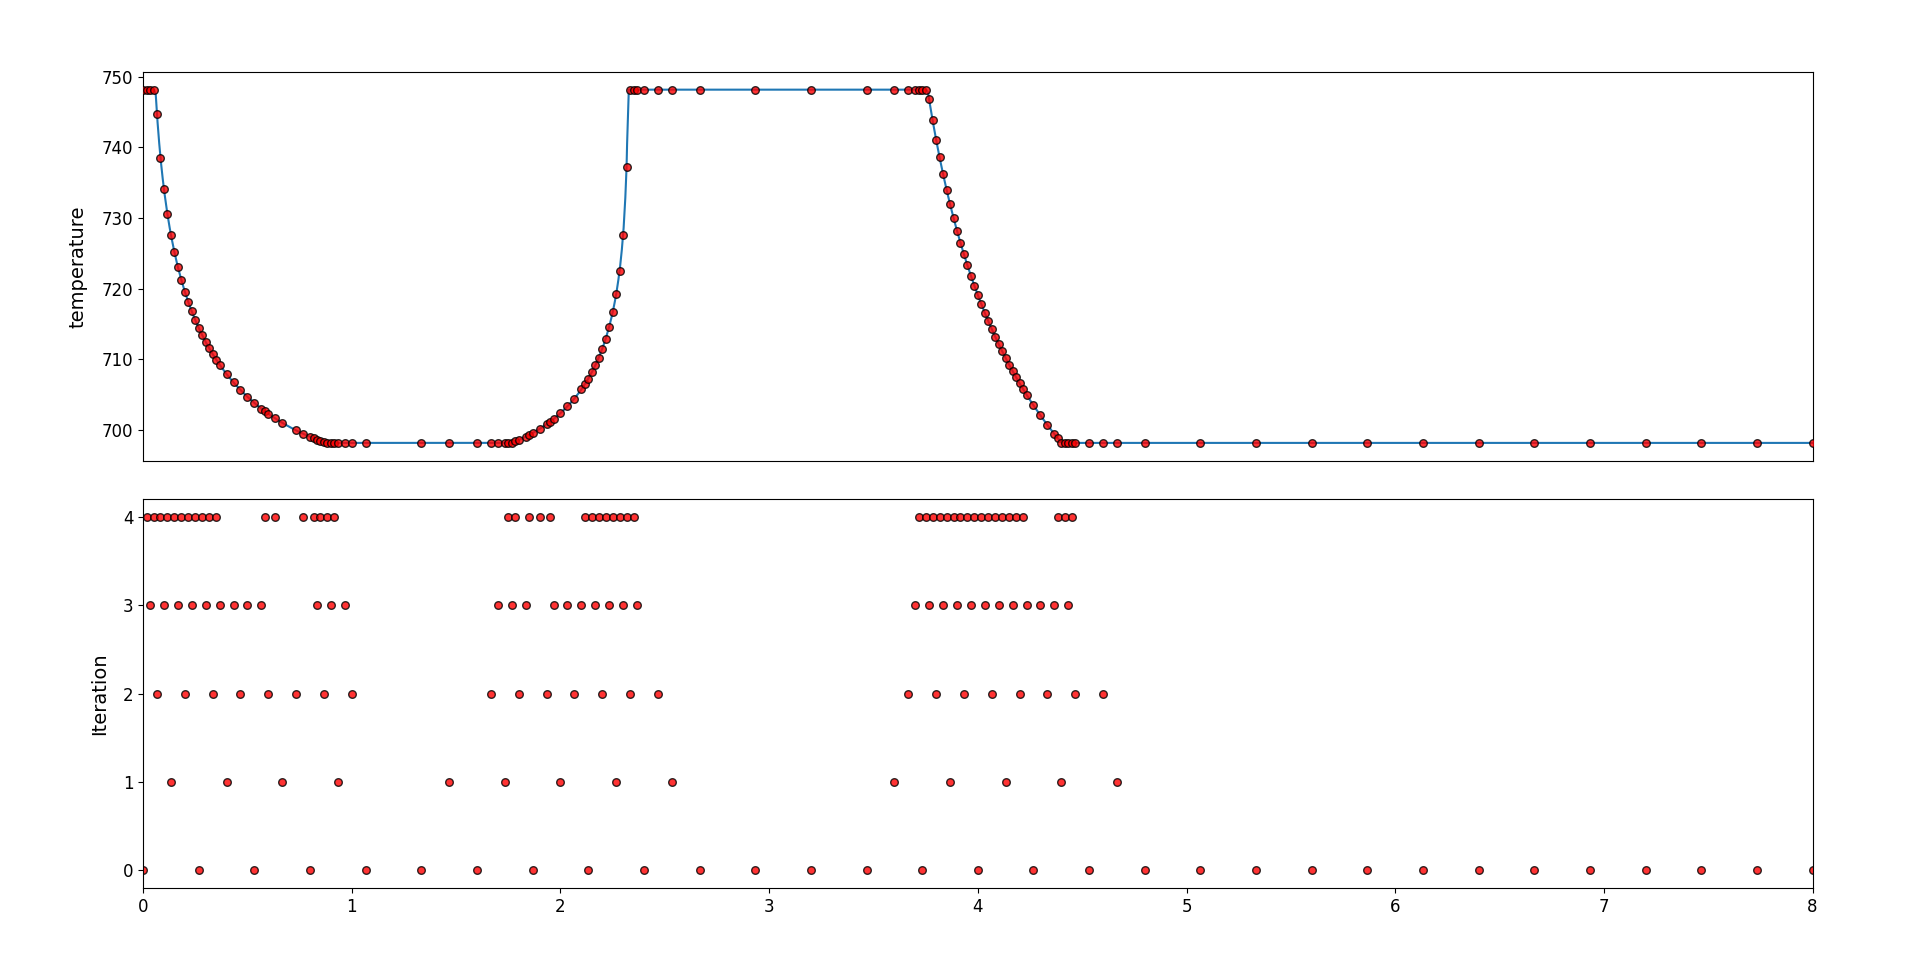
\includegraphics[width=1\textwidth]{images/refinement.png}\par\vspace{1cm}
	\vspace{2cm}

	{\large \textit{Author:}}\\[0.5em]
	{\large Linus Langenkamp}

	\vfill
	{\large \textit{Last updated on:}}\\[0.5em]
	{\large \today}

	\vspace*{1cm}
\end{titlepage}

\newpage
\fancyhead[R]{}
\thispagestyle{fancy}
\tableofcontents
\newpage

\fancyhead[R]{\leftmark}  % Restore right header

\clearpage
\pagestyle{fancy}
\setcounter{page}{1}

\section{Introduction}

Dynamic optimization is a branch of mathematical optimization that deals with
systems that evolve over time. The goal is to find optimal state trajectories
satisfying given differential equations by adjusting the controls over a
certain time horizon. These so-called optimal control problems are of great
importance in industrial applications and occur in various areas such as
industrial biochemistry, economics and aerospace engineering.

This guide presents a high level Python modeling environment for
solving dynamic optimization problems using local collocation methods and
adaptive mesh refinement techniques under the hood.
The following sections provide
step-by-step instructions on setting up, modeling and optimizing dynamic models
along with analyzing the optimal solution.

\subsection{Overview of the Framework} \label{c:overview}

The dynamic optimization framework, GDOPT, was developed to enable easy
modeling and optimization of dynamic systems. It consists of two main
components:

A Python front-end that provides the user with a high-level interface to model
the continuous problem and set flags, such as enabling mesh refinements or
setting tolerances.
A C++ back-end that performs the computationally intensive task of solving the
resulting large-scale nonlinear problem (NLP) with IPOPT (Interior Point
OPTimizer). In addition, a novel mesh refinement algorithm (L2-Boundary-Norm)
is implemented that performs an h-method. This leads to high-resolution
solutions at discontinuities, steep sections or corners of control variables.

The framework is very flexible and expressive, but retains a simple and
accessible syntax. The front-end has many special features that are presented
in this guide.

Once a dynamic optimization problem is defined, the framework discretizes it
and applies numerical techniques to transform it into a sparse NLP that can be
efficiently solved. In the following section, this process is described in
principal.

\subsection{How the Framework Solves Dynamic Models} \label{c:collocation}

The framework solves continuous dynamic optimization problems by discretizing
them over the specified time horizon. This is achieved by the following steps:

\begin{itemize}

	\item Time discretization:
	      The continuous time horizon is discretized into $N$ equidistant grid
	      points.

	\item {Dynamic constraints}:
	      Within each of the resulting intervals, a RadauIIA collocation scheme
	      is constructed, inserting $M = 1, \ldots, 36$ nodes on each interval.
	      Consequently, the states of the model are represented by a polynomial of degree
	      $M$ on each interval, discretizing the dynamics.

	\item {Non-dynamic constraints}:
	      Non-dynamic constraints are discretized at all nodes according to their
	      time frame. For example, path constraints must apply at every node and final
	      constraints at the very last node.

	\item {Objective function}:
	      The Lagrange term, which is an integral over the entire time horizon,
	      is approximated using the quadrature rule, which corresponds to the RadauIIA
	      collocation scheme.
	      The Mayer term, which represents a cost function evaluated at the last
	      time point, is replaced by an evaluation at the last node.

	\item {Transformation to a nonlinear problem}:
	      The local collocation-based discretization leads to a large-scale
	      nonlinear problem. This NLP has very sparse Jacobians and Hessians, which makes
	      it well suited for modern optimization algorithms.

	\item {Back-end solution}:
	      The C++ back-end of the framework solves this NLP with IPOPT. The
	      Python front-end allows access to this back-end so that the user can interact
	      with the solver via a series of flags. For example, if the number of mesh
	      refinement iterations is set greater than 0, the optimization and refinement
	      are looped, refining and optimizing the mesh sequentially. This provides a very
	      precise solution to the optimization problem.

\end{itemize}
This overall approach combines the flexibility of Python with the computational
efficiency of C++, ensuring that dynamic optimization problems can be solved
efficiently.

\section{Installation}

First, clone the GDOPT repository from GitHub:

\begin{lstlisting}[language=bash]
git clone https://github.com/linuslangenkamp/GDOPT.git
\end{lstlisting}

Depending on your operating system, follow the installation instructions.

\begin{mdframed}[backgroundcolor=gray!10, roundcorner=10pt,
		linewidth=1pt]

	\textbf{Ubuntu:}

	Make sure that the dependencies (git, curl, gfortran, LAPACK, CMake, g++,
	Python3, Python3-Venv, Python3-Build) are installed on the system.

	\begin{lstlisting}[language=bash]
sudo apt-get install git curl gfortran liblapack-dev cmake g++ python3 python3-venv
pip install build
\end{lstlisting}

	To keep the environment isolated, it is advised to create and activate a
	virtual environment:

	\begin{lstlisting}[language=bash]
python3 -m venv .venv
source .venv/bin/activate
\end{lstlisting}

	With the virtual environment activated, install the package. This will
	automatically install
	IPOPT\cite{wachter2006implementation}, the linear solver
	MUMPS\cite{amestoy2001fully}, and the Python packages used in the front-end,
	i.e. SymEngine\cite{symengine}, NumPy\cite{harris2020array},
	SciPy\cite{virtanen2020scipy}, pandas\cite{mckinney2010data}, and
	Matplotlib\cite{hunter2007matplotlib}:

	\begin{lstlisting}[language=bash]
pip install .
\end{lstlisting}
\end{mdframed}

Now it is possible to use GDOPT in your Python scripts:
\begin{lstlisting}[language=python]
import gdopt
\end{lstlisting}
In addition to MUMPS, linear solvers from the HSL suite such as MA27, MA57,
MA77, MA86, MA97\cite{hsl2013collection} may also be used if a license is
present. To do this, the environment variable “LIB\_HSL” must be set to the
corresponding path. The framework can then load the solvers at runtime.

\section{Getting Started}
This section shows how to set up and solve a simple dynamic
optimization problem with the proposed framework.

\subsection{Basic Example}
Here is a minimal working example for a bang-bang control problem, adapted from
the OpenModelica User's Guide \cite{openmodelica}
\begin{lstlisting}
from gdopt import *

model = Model("bangBang")

# states x1(t), x2(t) with x1(0) = x2(0) = 0
x1 = model.addState(start=0, symbol="obj") 
x2 = model.addState(start=0, symbol="obj'")

# control: u(t) with |u(t)| <= 10
u = model.addControl(lb=-10, ub=10, symbol="control") 

# dynamic: x1''(t) = u(t)
model.addDynamic(x1, x2) # x1'(t) = x2(t)
model.addDynamic(x2, u)  # x2'(t) = u(t)

# algebraic constraints
model.addPath(x2 * u, lb=-30, ub=30) # -30 <= x2(t) * u(t) <= 30
model.addFinal(x2, eq=0) # x2(tf) = 0

# objective = x1(tf) -> max
model.addMayer(x1, Objective.MAXIMIZE) 

# generate the C++ code
model.generate() 

# tf=0.5s, 150 intervals, using RadauIIA 3 step order 5 scheme
model.optimize(tf=0.5, steps=150, rksteps=3)

model.plot()
	\end{lstlisting}

\subsection{Explanation}
Example procedure:
\begin{itemize}
	\item Import the package and create a \texttt{Model} object
	      with a given name
	\item Add the states with given starting values (and optionally
	      assign a symbol)
	\item Add the control with lower and upper bounds (and
	      optionally assign a symbol)
	\item Define the dynamic, path, final constraints
	\item Add an objective
	\item Generate the C++ code
	\item Optimize for a given final time, number of steps and
	      collocation nodes
	\item Plot the model
\end{itemize}

\begin{figure}[H]
	\centering
	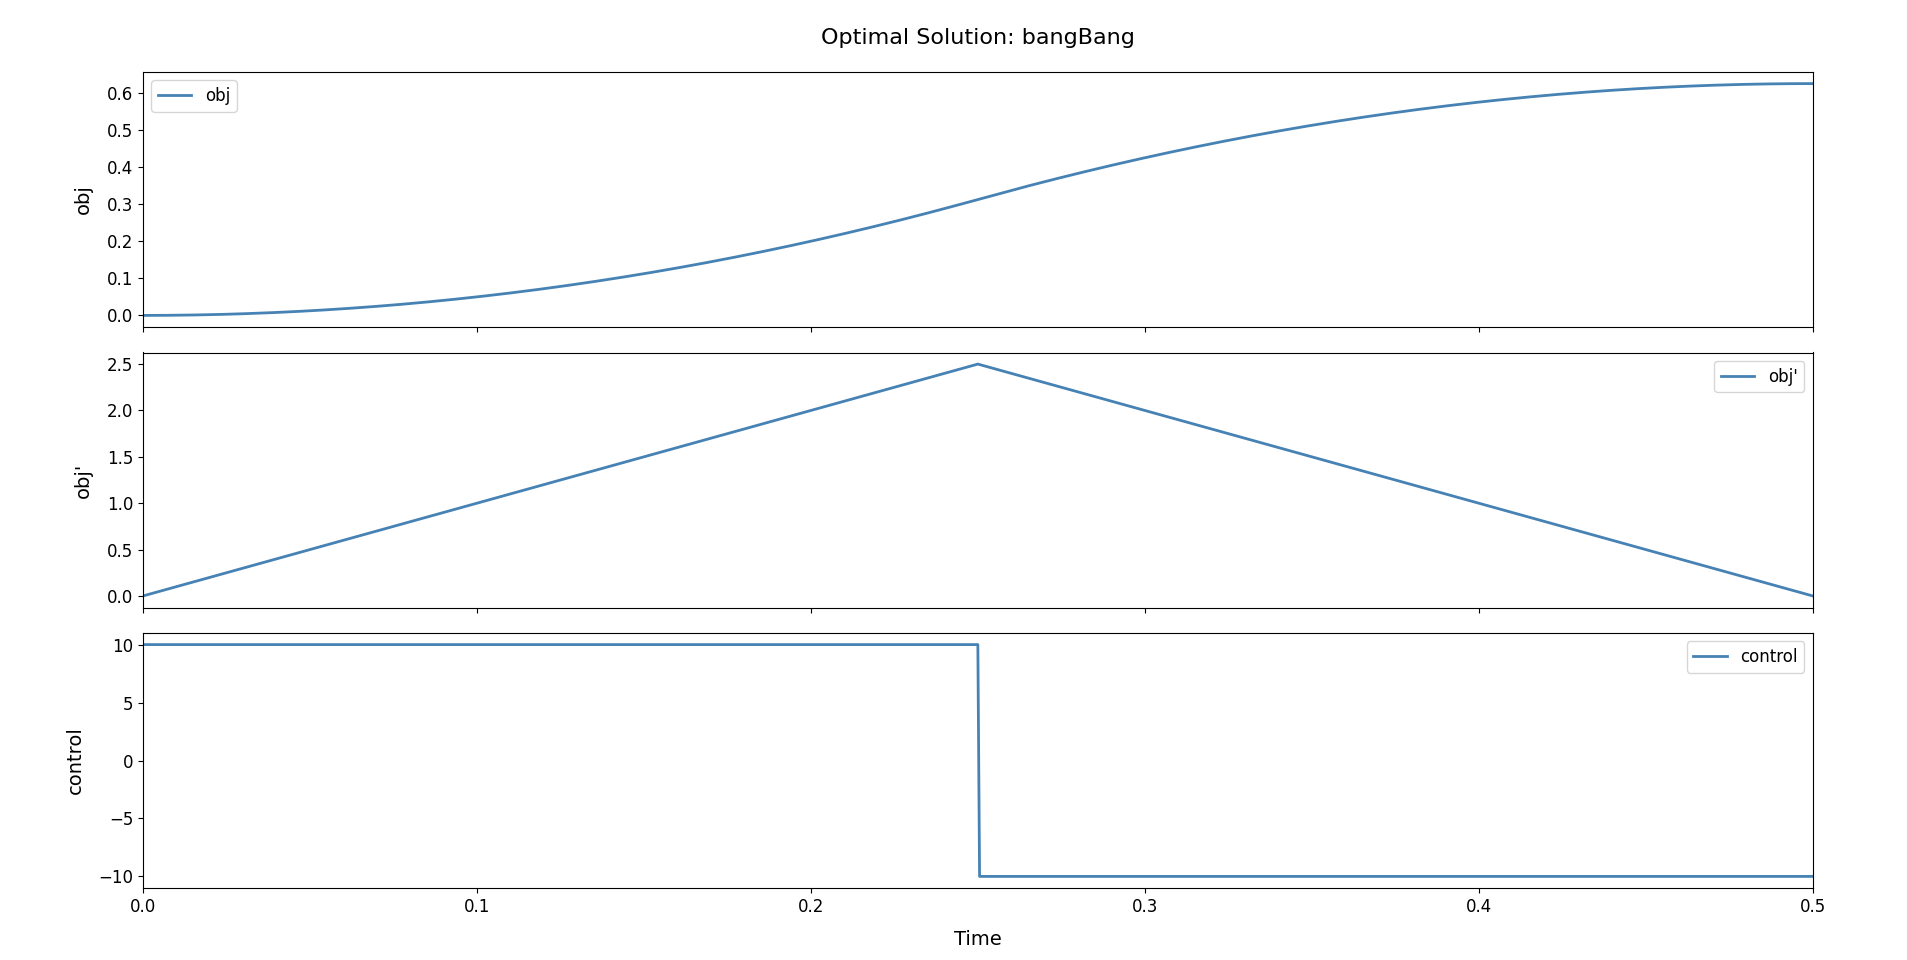
\includegraphics[width=\textwidth]{images/bangBang.png}
	\caption{Optimal bang-bang solution provided by the framework}
	\label{fig:bangBang}
\end{figure}
\section{Mathematical Problem Formulation}
\label{c:GDOP}

In a \textbf{General Dynamic Optimization Problem} (GDOP) the goal is the
minimization of a \textit{Mayer term}, which defines the cost at the final time
$t_f$ (terminal cost), and a \textit{Lagrange term}, which represents the
running cost over the time horizon $[t_0, t_f]$. The problem can be written as
follows:

\begin{equation*}
	\min_{\v{u}(t), \v{p}} \quad \underbrace{M(\v{x}(t_f), \v{u}(t_f),
		\v{p}, t_f)}_{\text{Mayer term}} + \underbrace{\int_{t_0}^{t_f} L(\v{x}(t),
		\v{u}(t), \v{p}, t)\, \dd t}_{\text{Lagrange term}}
\end{equation*}

subject to the following constraints:

\begin{itemize}
	\item \textit{Dynamic constraints}:
	      The states of the system are evaluated by the differential equation
	      $\dot{\v{x}}(t) = \v{f}(\v{x}(t), \v{u}(t), \v{p}, t)$. The differential
	      equation must apply for all times $t \in [t_0, t_f]$ and has the initial
	      condition $\v{x}(t_0) = \v{x}_0$.

	\item \textit{Path constraints}:
	      For all times $t \in [t_0, t_f]$, the variables must satisfy the
	      inequality $\v{g}^L \leq \v{g}(\v{x}(t), \v{u}(t), \v{p}, t) \leq \v{g}^U$.
	      These may represent physical restrictions, for example.

	\item \textit{Final constraints}:
	      At the final time $t_f$, $\v{r}^L \leq \v{r}(\v{x}(t_f), \v{u}(t_f),
		      \v{p}, t_f) \leq \v{r}^U$ must be fulfilled. These constraints define the
	      desired final configuration of the system.

	\item \textit{Parametric constraints:}
	      The static parameters must satisfy the algebraic inequality constraints
	      $\v{a}^L \leq \v{a}(\v{p}) \leq \v{a}^U$.
\end{itemize}

\noindent
\textbf{Variables and Functions:}
\begin{itemize}
	\item $t$: Time in the model.
	\item $t_f$: Final time of the time horizon.
	\item $\v{x}(t)$: States, which evolve according to the dynamics
	      $\dot{\v{x}}(t) = \v{f}(\cdot)$.
	\item $\v{u}(t)$: Time-dependent control variables, also referred to as
	      inputs.
	\item $\v{p}$: Static parameters.
	\item $M(\cdot)$: Mayer term, a function that evaluates a cost at the
	      final time.
	\item $L(\cdot)$: Lagrange integrand, a function defining a cost at a
	      specific time $t$. $\int_{t_0}^{t_f} L(\cdot) \, \dd t$ is then referred to as
	      the Lagrange term.
	\item $\v{f}(\cdot)$: Function defining the system dynamics.
	\item $\v{g}(\cdot)$: Path constraint function, which forces
	      restrictions on variables at all times.
	\item $\v{r}(\cdot)$: Final constraint function, which forces
	      restrictions on variables at the final time.
	\item $\v{a}(\cdot)$: Parametric constraint function, which forces
	      restrictions on solely static parameters.
\end{itemize}

In this problem formulation, the goal is to minimize the combined objective of
the Mayer and Lagrange terms while ensuring that the system dynamics, path
constraints, final constraints, and parametric constraints are all satisfied.

The entire problem can be formulated in standard notation as
\begin{align*}
	\min_{\v{u}(t), \v{p}} ~ & M(\v{x}(t_f), \v{u}(t_f),
	\v{p}, t_f) + \int_{t_0}^{t_f} L(\v{x}(t), \v{u}(t), \v{p}, t)
	\, \mathrm{d}t
	\\
	\text{s.t.}              &
	\\
	\dot{\v{x}}(t)           & = \v{f}(\v{x}(t), \v{u}(t), \v{p},
	t)\
	\forall t \in [t_0, t_f]
	\\
	\v{x}(t_0)               & = \v{x}_0
	\\
	\v{g}^{L}                & \leq \v{g}(\v{x}(t), \v{u}(t),
	\v{p}, t)
	\leq \v{g}^{U}\ \forall t \in [t_0, t_f]
	\\
	\v{r}^{L}                & \leq \v{r}(\v{x}(t_f), \v{u}(t_f),
	\v{p},
	t_f) \leq \v{r}^{U}
	\\
	\v{a}^{L}                & \leq \v{a}(\v{p}) \leq \v{a}^{U}
\end{align*}
where $L, M, \v{f}, \v{g}, \v{r}, \v{a} \in C^2$, i.e. are continuously
differentiable twice.

\section{Modeling}

\subsection{Model Creation}
The first step is to create a new Python file and to import the
\texttt{gdopt} package.
\begin{lstlisting}
from gdopt import *
	\end{lstlisting}

Additionally a \texttt{Model} object has to be created, which is the basis for
all modeling.

\begin{mdframed}[backgroundcolor=gray!10, roundcorner=10pt, linewidth=1pt]

	Constructs a \texttt{Model} object.

	\begin{lstlisting}
model = Model(name="DummyName")
	\end{lstlisting}\label{Model}

	\textbf{Parameters:}
	\begin{itemize}
		\item \texttt{str name} \emph{(optional)}: The name of the
		      model.
	\end{itemize}

	\textbf{Returns:}
	\texttt{Model model}: The \texttt{Model} object.

	\textbf{Example:}
	\begin{lstlisting}
model = Model("Model Name")
	\end{lstlisting}
\end{mdframed}

The variables, constraints and objectives are added to this
\texttt{Model} object. Note that a \texttt{Model} can be printed to the
standard output with the native \texttt{print} function.

\subsection{Variables}

\subsubsection{States}

States are time-dependent functions, that are calculated in the
solving process. The value of the state is completely determined by a starting
value and an ordinary differential equation.

\begin{mdframed}[backgroundcolor=gray!10, roundcorner=10pt, linewidth=1pt]

	Adding a state to a \texttt{Model} object.

	\begin{lstlisting}
x = model.addState(start, symbol=None, lb=-float("inf"), ub=float("inf"), nominal=None)
	\end{lstlisting}\label{addState}

	\textbf{Parameters:}
	\begin{itemize}
		\item \texttt{float start}: The initial value of the state
		      variable.
		\item \texttt{str symbol} \emph{(optional)}: A symbolic
		      representation of the state. The state is
		      represented by this symbol in
		      further analysis.
		\item \texttt{float lb} \emph{(optional)}: Lower bound for the
		      state variable.
		\item \texttt{float ub} \emph{(optional)}: Upper bound for the
		      state variable.
		\item \texttt{float nominal} \emph{(optional)}: A nominal value
		      for scaling.
	\end{itemize}

	\textbf{Returns:}
	\texttt{Symbol variable}: The symbolic representation of the state
	variable, which can be used in constraints.

	\textbf{Aliases:} \texttt{model.addX}
\end{mdframed}

\subsubsection{Inputs}

Input or controls are time-dependent functions, that are calculated in the
solving process and are not differentiated in the model.

\begin{mdframed}[backgroundcolor=gray!10, roundcorner=10pt, linewidth=1pt]

	Adding an input / control variable $u(t)$, that changes over time, to a
	\texttt{Model} object.

	\begin{lstlisting}
u = model.addInput(symbol=None, lb=-float("inf"), ub=float("inf"), guess=0, nominal=None)
	\end{lstlisting}
	\label{addInput}
	\textbf{Parameters:}
	\begin{itemize}
		\item \texttt{str symbol} \emph{(optional)}: A symbolic
		      representation of the input. The input is
		      represented by this symbol in
		      further analysis.
		\item \texttt{float lb} \emph{(optional)}: Lower bound for the
		      input variable.
		\item \texttt{float ub} \emph{(optional)}: Upper bound for the
		      input variable.
		\item \texttt{Expression guess} \emph{(optional)}: An initial
		      guess for the input. Further explanation in
		      \eqref{p:cguesses}.
		\item \texttt{float nominal} \emph{(optional)}: A nominal value
		      for scaling.
	\end{itemize}

	\textbf{Returns:}
	\texttt{Symbol variable}: The symbolic representation of the input,
	which can be used in constraints.

	\textbf{Aliases:}  \texttt{model.addU}, \texttt{model.addControl},
	\texttt{model.addContinuous}
\end{mdframed}

\paragraph{Input Guesses}
\label{p:cguesses}
The guess parameter in \texttt{model.addInput} \eqref{addInput} can be
any \texttt{Expression} that contains the global time or final time symbols
\eqref{c:globaltime}, but can also be a regular constant \texttt{float} or
\texttt{int}. If the \texttt{"initVars"} flag \eqref{flag:initVars} is chosen
to be a
\texttt{SOLVE} option \eqref{enum:initVars}, this trajectory is used to
solve the dynamic and provide an initial, feasible guess for the state
variables. If the option \texttt{InitVars.CONST} is set, the guess is used
nevertheless, although the states are initialized constant. Note that any valid
SymEngine \texttt{Expression} can be provided as
a guess, although there are several standard functions to provide better
initial guesses for the control.

\begin{mdframed}[backgroundcolor=gray!10, roundcorner=10pt, linewidth=1pt]

	Providing a constant control guess trajectory.

	\begin{lstlisting}
guessConstant(const)
	\end{lstlisting}

	\textbf{Parameters:}
	\begin{itemize}
		\item \texttt{float const}: Constant value for the control
		      guess, i.e. $u(t) \equiv const ~ \forall t \in [0, t_f]$.
	\end{itemize}

	\textbf{Remarks:} It's also possible to just write \texttt{guess=const}
	in the \texttt{model.addInput} arguments.
\end{mdframed}

\begin{mdframed}[backgroundcolor=gray!10, roundcorner=10pt, linewidth=1pt]

	Providing a linear control guess trajectory. The provided values are
	interpolated accordingly.

	\begin{lstlisting}
guessLinear(u0, uf)
	\end{lstlisting}

	\textbf{Parameters:}
	\begin{itemize}
		\item \texttt{float u0}: Value for the control guess at $t=0$,
		      i.e. $u(0)$.
		\item \texttt{float uf}: Value for the control guess at
		      $t=t_f$, i.e. $u(t_f)$.
	\end{itemize}

\end{mdframed}

\begin{mdframed}[backgroundcolor=gray!10, roundcorner=10pt, linewidth=1pt]

	Providing a quadratic control guess trajectory. The provided values
	are interpolated accordingly.

	\begin{lstlisting}
guessQuadratic(u0, um, uf)
	\end{lstlisting}

	\textbf{Parameters:}
	\begin{itemize}
		\item \texttt{float u0}: Value for the control guess at $t=0$,
		      i.e. $u(0)$.
		\item \texttt{float um}: Value for the control guess at
		      $t=\frac{t_f}{2}$, i.e. $u(\frac{t_f}{2})$.
		\item \texttt{float uf}: Value for the control guess at
		      $t=t_f$, i.e. $u(t_f)$.
	\end{itemize}

\end{mdframed}

\begin{mdframed}[backgroundcolor=gray!10, roundcorner=10pt, linewidth=1pt]

	Providing an exponential control guess trajectory. The provided values
	are interpolated accordingly.

	\begin{lstlisting}
guessExponential(u0, uf)
	\end{lstlisting}

	\textbf{Parameters:}
	\begin{itemize}
		\item \texttt{float u0}: Value for the control guess at $t=0$,
		      i.e. $u(0)$.
		\item \texttt{float uf}: Value for the control guess at
		      $t=t_f$, i.e. $u(t_f)$.
	\end{itemize}

\end{mdframed}

\begin{mdframed}[backgroundcolor=gray!10, roundcorner=10pt, linewidth=1pt]

	Providing a piecewise defined control guess trajectory.

	\begin{lstlisting}
guessPiecewise(*args)
	\end{lstlisting}

	\textbf{Parameters:}
	\begin{itemize}
		\item \texttt{*(Expression, Condition) *args}: Arbitrary number
		      of tuples. The first argument in each tuple has to be an
		      \texttt{Expression} and the second argument is the corresponding interval its
		      defined on.

	\end{itemize}

	\textbf{Example:} \texttt{guessPiecewise((0.6, t <= 0.5), (2 + t**2,
		0.5 < t))} represents the initial control guess $u(t) =
		\begin{cases}
			0.6,     & t \leq \frac{1}{2} \\
			2 + t^2, & t > \frac{1}{2}
		\end{cases}$. Note that these expressions can be standard
	expressions
	such as \texttt{guessQuadratic}, \texttt{guessLinear} or any arbitrary
	SymEngine \texttt{Expression}.
\end{mdframed}

\subsubsection{Parameters}

Parameters are time-invariant constants, that are calculated in the
solving process.

\begin{mdframed}[backgroundcolor=gray!10, roundcorner=10pt,
		linewidth=1pt]

	Adding a parameter variable, that is time-invariant constant,
	to a \texttt{Model} object.

	\begin{lstlisting}
p = model.addParameter(symbol=None, lb=-float("inf"), ub=float("inf"), guess=0, nominal=None)
		\end{lstlisting}
	\label{addParameter}
	\textbf{Parameters:}
	\begin{itemize}
		\item \texttt{str symbol} \emph{(optional)}: A symbolic
		      representation of the parameter. The parameter is
		      represented by this
		      symbol in further analysis.
		\item \texttt{float lb} \emph{(optional)}: Lower bound
		      for the parameter variable.
		\item \texttt{float ub} \emph{(optional)}: Upper bound
		      for the parameter variable.
		\item \texttt{Expression guess} \emph{(optional)}: An
		      initial guess for the parameter.
		\item \texttt{float nominal} \emph{(optional)}: A
		      nominal value for scaling.
	\end{itemize}

	\textbf{Returns:}
	\texttt{Symbol variable}: The symbolic representation of the
	parameter, which can be used in constraints.

	\textbf{Aliases:} \texttt{model.addP}
\end{mdframed}

\subsubsection{Runtime Parameters}
\label{c:runtimeParameters}
Runtime parameters are time-invariant global constants, that can be
changed after code generation and compilation via \texttt{model.setValue}. The
value of the
runtime parameter will be set at runtime. These represent usual
parameters of standard modeling environments. A runtime parameter can be used
literally anywhere in the \texttt{Model} object, e.g. in objectives or
constraints, as a starting value, a lower or upper bound and even as a nominal
value.

\begin{mdframed}[backgroundcolor=gray!10, roundcorner=10pt,
		linewidth=1pt]

	Adding a runtime parameter to the model. This is a constant in
	the model, that will be substituted by its associated value at runtime
	time.

	\begin{lstlisting}
rp = model.addRuntimeParameter(default, symbol=None)
		\end{lstlisting}
	\label{addRuntimeParameter}
	\textbf{Parameters:}
	\begin{itemize}
		\item \texttt{float default}: A default value for the
		      runtime parameter.
		\item \texttt{str symbol} \emph{(optional)}: A symbolic
		      representation of
		      the runtime parameter.
	\end{itemize}

	\textbf{Returns:}
	\texttt{Symbol variable}: The symbolic representation of the
	runtime parameter.

	\textbf{Aliases:} \texttt{model.addRP}
\end{mdframed}

\begin{mdframed}[backgroundcolor=gray!10, roundcorner=10pt,
		linewidth=1pt]

	Changing the associated value of a runtime parameter.

	\begin{lstlisting}
model.setValue(runtimeParameter, value)
		\end{lstlisting}
	\label{setValue}
	\textbf{Parameters:}
	\begin{itemize}
		\item \texttt{Symbol runtimeParameter}: A symbolic
		      representation of the runtime parameter.
		\item \texttt{float value}: The new associated value
		      for the runtime parameter.
	\end{itemize}
\end{mdframed}

\subsection{Constraints}

Any constraint can contain runtime constants such as the global
final time \eqref{finalTimeSymbol} or runtime parameters
\eqref{c:runtimeParameters}.

\subsubsection{Dynamic Constraints}

Dynamic constraints are explicit ordinary differential equations with
the derivative of a state on the left hand side and the corresponding rate of
change on the right hand side. This equation must hold at every moment.

\begin{mdframed}[backgroundcolor=gray!10, roundcorner=10pt,
		linewidth=1pt]

	Adding a dynamic constraint $\frac{\dd y(t)}{\dd t} =
		f(\v{x}(t), \v{u}(t), \v{p}, t) \,\, \forall t \in [t_0, t_f]$
	to
	the \texttt{Model}
	object, where $y(t)$ is a previously added state.

	\begin{lstlisting}
model.addDynamic(diffVar, expr, nominal=None)
		\end{lstlisting}
	\label{addDynamic}
	\textbf{Parameters:}
	\begin{itemize}
		\item \texttt{Symbol diffVar}: The state variable that
		      gets differentiated, i.e. $y(t)$.
		\item \texttt{Expression expr}: The right hand side of
		      the ordinary differential equation, i.e. $f(\cdot)$.
		\item \texttt{float nominal} \emph{(optional)}: A
		      nominal value of $f(\cdot)$ for scaling.
	\end{itemize}

	\textbf{Aliases:}  \texttt{model.addF}, \texttt{model.addOde}

	\textbf{Example:} \texttt{model.addDynamic(x1, x1 * u1 + p +
		t)} represents the differential equation
	$\frac{\dd x_1(t)}{\dd t} = x_1(t) u_1(t) + p + t$. (Using the
	global time symbol \eqref{c:globaltime})
\end{mdframed}

\subsubsection{Path Constraints}

Path constraints are algebraic constraints on states, inputs,
parameters and time, that must hold at every moment.

\begin{mdframed}[backgroundcolor=gray!10, roundcorner=10pt,
		linewidth=1pt]

	Adding a path constraint ${g}^{L} \leq {g}(\v{x}(t), \v{u}(t),
		\v{p}, t) \leq {g}^{U}\ \forall t \in [t_0, t_f]$ to the
	\texttt{Model} object.

	\begin{lstlisting}
model.addPath(expr, lb=-float("inf"), ub=float("inf"), eq=None, nominal=None)
		\end{lstlisting}
	\label{addPath}
	\textbf{Parameters:}
	\begin{itemize}
		\item \texttt{Expression expr}: The algebraic
		      expression, i.e. $g(\cdot)$.
		\item \texttt{float lb} \emph{(optional)}: Lower bound
		      for the path constraint.
		\item \texttt{float ub} \emph{(optional)}: Upper bound
		      for the path constraint.
		\item \texttt{float eq} \emph{(optional)}: Equality
		      parameter for the path constraint. Can not be chosen
		      simultaneously with
		      \texttt{lb} nor \texttt{ub}.
		\item \texttt{float nominal} \emph{(optional)}: A
		      nominal value of $g(\cdot)$ for scaling.
	\end{itemize}

	\textbf{Aliases:}  \texttt{model.addG}

	\textbf{Example:} \texttt{model.addPath(x1**2 + u1**2, ub=5)}
	represents the path constraint
	$x_1^2 + u_1^2 \leq 5$.
\end{mdframed}

\subsubsection{Final Constraints}

Final constraints are algebraic constraints on states, control and
parameters, that must hold at the final time $t_f$.

\begin{mdframed}[backgroundcolor=gray!10, roundcorner=10pt,
		linewidth=1pt]

	Adding a final constraint ${r}^{L} \leq {r}(\v{x}(t_f),
		\v{u}(t_f), \v{p}, t_f) \leq {r}^{U}$ to the \texttt{Model}
	object.

	\begin{lstlisting}
model.addFinal(expr, lb=-float("inf"), ub=float("inf"), eq=None, nominal=None)
		\end{lstlisting}
	\label{addFinal}
	\textbf{Parameters:}
	\begin{itemize}
		\item \texttt{Expression expr}: The algebraic
		      expression, i.e. $r(\cdot)$.
		\item \texttt{float lb} \emph{(optional)}: Lower bound
		      for the final constraint.
		\item \texttt{float ub} \emph{(optional)}: Upper bound
		      for the final constraint.
		\item \texttt{float eq} \emph{(optional)}: Equality
		      parameter for the final constraint. Can not be chosen
		      simultaneously with
		      \texttt{lb} nor \texttt{ub}.
		\item \texttt{float nominal} \emph{(optional)}: A
		      nominal value of $r(\cdot)$ for scaling.
	\end{itemize}

	\textbf{Aliases:}  \texttt{model.addR}

	\textbf{Example:} \texttt{model.addFinal(x1 + u1 - p, eq=0)}
	represents the final constraint
	$x_1(t_f) + u_1(t_f) - p = 0$.
\end{mdframed}

\subsubsection{Parametric Constraints}

Parametric constraints are algebraic constraints that can
contain only parameters.

\begin{mdframed}[backgroundcolor=gray!10, roundcorner=10pt,
		linewidth=1pt]

	Adding a parametric constraint ${a}^{L} \leq {a}(\v{p}) \leq
		{a}^{U}$ to the \texttt{Model} object.

	\begin{lstlisting}
model.addParametric(expr, lb=-float("inf"), ub=float("inf"), eq=None, nominal=None)
		\end{lstlisting}
	\label{addParametric}
	\textbf{Parameters:}
	\begin{itemize}
		\item \texttt{Expression expr}: The algebraic
		      expression, i.e. $a(\cdot)$.
		\item \texttt{float lb} \emph{(optional)}: Lower bound
		      for the parametric constraint.
		\item \texttt{float ub} \emph{(optional)}: Upper bound
		      for the parametric constraint.
		\item \texttt{float eq} \emph{(optional)}: Equality
		      parameter for the parametric constraint. Can not be
		      chosen simultaneously with
		      \texttt{lb} nor \texttt{ub}.
		\item \texttt{float nominal} \emph{(optional)}: A
		      nominal value of $a(\cdot)$ for scaling.
	\end{itemize}

	\textbf{Aliases:}  \texttt{model.addA}

	\textbf{Example:} \texttt{model.addParametric(sin(p1) -
		p2, lb=0)} represents the parametric constraint
	$0 \leq \sin(p_1) - p_2$.
\end{mdframed}

\subsection{Objective}

Any objective can contain runtime constants such as the global
final time \eqref{finalTimeSymbol} or runtime parameters
\eqref{c:runtimeParameters}.

\subsubsection{Mayer Term}

The Mayer term penalizes the final configuration of the system.

\begin{mdframed}[backgroundcolor=gray!10, roundcorner=10pt,
		linewidth=1pt]

	Adding a Mayer term $M(\v{x}(t_f), \v{u}(t_f), \v{p}, t_f)$ to
	the \texttt{Model} object.

	\begin{lstlisting}
model.addMayer(expr, obj=Objective.MINIMIZE, nominal=None)
		\end{lstlisting}
	\label{addMayer}
	\textbf{Parameters:}
	\begin{itemize}
		\item \texttt{Expression expr}: The Mayer term, i.e.
		      $M(\cdot)$.
		\item \texttt{Objective obj} \emph{(optional)}: The
		      objective goal for the Mayer term, corresponding to an
		      element of the objective
		      enumeration \eqref{enum:Objective}.
		\item \texttt{float nominal} \emph{(optional)}: A
		      nominal value of $M(\cdot)$ for scaling.
	\end{itemize}

	\textbf{Aliases:}  \texttt{model.addM}

	\textbf{Example:} \texttt{model.addMayer(x1 + x2**2,
		obj=Objective.MINIMIZE)} represents the Mayer term
	$x_1 + x_2^2$.
\end{mdframed}

\subsubsection{Lagrange Term}

The Lagrange term defines a cumulative cost of the system over the
entire time horizon.

\begin{mdframed}[backgroundcolor=gray!10, roundcorner=10pt,
		linewidth=1pt]

	Adding a Lagrange term $\int_{t_0}^{t_f} L(\v{x}(t), \v{u}(t),
		\v{p}, t) \, \mathrm{d}t$ to the \texttt{Model} object.

	\begin{lstlisting}
model.addLagrange(expr, obj=Objective.MINIMIZE, nominal=None)
	 	\end{lstlisting}
	\label{addLagrange}
	\textbf{Parameters:}
	\begin{itemize}
		\item \texttt{Expression expr}: The Lagrange integrand,
		      i.e. $L(\cdot)$.
		\item \texttt{Objective obj} \emph{(optional)}: The
		      objective goal for the Lagrange term, corresponding to an
		      element of the
		      objective enumeration \eqref{enum:Objective}.
		\item \texttt{float nominal} \emph{(optional)}: A
		      nominal value of $L(\cdot)$ for scaling.
	\end{itemize}

	\textbf{Aliases:}  \texttt{model.addL}

	\textbf{Example:} \texttt{model.addLagrange(x1 * u1 + t,
		obj=Objective.MINIMIZE)} represents the Lagrange term
	$\int_{t_0}^{t_f} x_1(t) u_1(t) + t \, \mathrm{d}t$.
\end{mdframed}

\subsubsection{Combined Objectives}

If both the Mayer and Lagrange term are contained in a model, there are
specific factors that must be taken into account. The objective goal
\texttt{obj} is multiplying the associated term with a factor of $-1$, if
maximization is chosen. If these goals differ between both terms, e.g. $\max
	M(\cdot)$ and $\min  \int_{t_0}^{t_f} L(\cdot) \, \dd t$, then the full
objective is given by $\min -M(\cdot) + \int_{t_0}^{t_f} L(\cdot) \, \dd t$ and
vice versa. Additionally nominal values are added if both terms have
assigned nominals. If only one term has a nominal value, then this value is
used for the full objective.

Combined objectives can be added individually with \texttt{model.addMayer}
\eqref{addMayer} and \texttt{model} \, \texttt{.addLagrange}
\eqref{addLagrange} or
with the method
\texttt{model.addObjective}.

\begin{mdframed}[backgroundcolor=gray!10, roundcorner=10pt,
		linewidth=1pt]

	Adding a Mayer $M(\v{x}(t_f), \v{u}(t_f), \v{p}, t_f)$ and
	Lagrange term $\int_{t_0}^{t_f} L(\v{x}(t), \v{u}(t), \v{p}, t) \,
		\mathrm{d}t$
	to the \texttt{Model} object.

	\begin{lstlisting}
model.addObjective(mayer, lagrange, obj=Objective.MINIMIZE, nominal=None)
		\end{lstlisting}
	\label{addObjective}
	\textbf{Parameters:}
	\begin{itemize}
		\item \texttt{Expression mayer}: The Mayer term, i.e.
		      $M(\cdot)$.
		\item \texttt{Expression lagrange}: The Lagrange
		      integrand, i.e. $L(\cdot)$.
		\item \texttt{Objective obj} \emph{(optional)}: The
		      objective goal for the combined cost of $M(\cdot) +
			      \int_{t_0}^{t_f} L(\cdot)
			      \, \dd t$, corresponding to an element of the
		      objective enumeration
		      \eqref{enum:Objective}.
		\item \texttt{float nominal} \emph{(optional)}: A
		      nominal value of the full objective for scaling.
	\end{itemize}

	\textbf{Example:} \texttt{model.addObjective(x1, x2 * u1,
		obj=Objective.MINIMIZE)} represents the full objective
	$x_1(t_f) + \int_{t_0}^{t_f} x_2(t) u_1(t) \, \mathrm{d}t$.
\end{mdframed}

\subsection{Code Generation}

If the modeling process is done, it is possible to generate and compile the C++
code of the
model.
Therefore, the 1st and 2nd derivatives of the objectives and all constraints
are calculated symbolically with SymEngine. After that, the framework will
search for common subexpressions (CSE) in each derivative, using the symbolic
capabilities of SymEngine. The resulting expressions as well as all other
problem defining structures are generated to a C++ file. This file makes
use of runtime constants / model parameters (e.g. final time, runtime
parameters, flags, paths,
\ldots), that will be set later in the \texttt{model.optimize} pipeline
\eqref{optimize}. The resulting C++ file is
compiled, while linking against the dynamic optimization back-end.

If several optimizations have to be executed, where only flags and runtime
parameters are changed, it is advised to call \texttt{model.generate} only
once, since all flags will be set in a later stage. Thus, obsolete
recalculations can be avoided.

\begin{mdframed}[backgroundcolor=gray!10, roundcorner=10pt,
		linewidth=1pt]

	Calculates the 1st and 2nd derivatives, generates all the problem
	defining structures to a .cpp file, and compiles the code.

	\begin{lstlisting}
model.generate()
\end{lstlisting}

\end{mdframed}

\subsection{Optimization}
After code generation and compilation, all model parameters (e.g. final time,
runtime
parameters, flags, paths, \ldots) have to be written to a configuration file.
The already existing executable will read in the configuration and then solve
the NLP. Additionally the optimal solution
as well as some metadata can be written to text files. These files can be
analyzed with the presented framework \eqref{c:Analysis}.

\begin{mdframed}[backgroundcolor=gray!10, roundcorner=10pt,
		linewidth=1pt]

	Sets all model parameters (e.g. final time, runtime parameters, flags,
	paths, \ldots) in the configuration file and runs the optimization.

	\begin{lstlisting}
model.optimize(tf=1, steps=1, rksteps=1, flags={}, meshFlags={}, resimulate=False, recompile=False)
	\end{lstlisting}
	\label{optimize}
	\textbf{Parameters:}
	\begin{itemize}
		\item \texttt{float tf} \emph{(optional)}: The final time $t_f$
		      of the model.
		\item \texttt{int steps} \emph{(optional)}: The number of
		      intervals.
		\item \texttt{int rksteps} \emph{(optional)}: The number of
		      collocation nodes of the RadauIIA integrator per
		      interval. Valid range: $1
			      \leq$ \texttt{rksteps} $\leq 36$.
		\item \texttt{dict<str, arg> flags} \emph{(optional)}: A
		      dictionary of flags. All possible flags are presented in
		      \eqref{c:flags}.
		\item \texttt{dict<str, arg> meshFlags} \emph{(optional)}: A
		      dictionary of mesh flags. All possible mesh flags are
		      presented in
		      \eqref{c:meshflags}.
		\item \texttt{bool resimulate} \emph{(optional)}: If set to
		      \texttt{true}, all arguments and flags of this method
		      will be taken from the
		      previous optimization.
	\end{itemize}

	\textbf{Example}:
	\begin{lstlisting}
model.optimize(
	tf=1,
	steps=250,
	rksteps=3,
	flags={
		"outputPath": "/tmp",
		"linearSolver": LinearSolver.MUMPS,
		"initVars": InitVars.SOLVE_EXPLICIT,
		"exportJacobianPath": "/tmp",
	},
	meshFlags={
		"algorithm": MeshAlgorithm.L2_BOUNDARY_NORM,
		"iterations": 6
	}
)
	\end{lstlisting}

\end{mdframed}

If \texttt{optimize} has to be called only once, it is also possible to use
\texttt{model.solve}. This is a basic wrapper, that calls \texttt{generate} and
\texttt{optimize} sequentially and shares the parameters with
\texttt{optimize}.

\begin{mdframed}[backgroundcolor=gray!10, roundcorner=10pt,
		linewidth=1pt]

	Generates all problem defining structures to a .cpp file, compiles,
	sets all model parameters (e.g. final time, runtime parameters, flags,
	paths, \ldots), and runs the optimization.

	\begin{lstlisting}
model.solve(tf=1, steps=1, rksteps=1, flags={}, meshFlags={}, resimulate=False)
	\end{lstlisting}
	\label{solve}
	\textbf{Parameters:}
	\begin{itemize}
		\item \texttt{float tf} \emph{(optional)}: The final time $t_f$
		      of the model.
		\item \texttt{int steps} \emph{(optional)}: The number of
		      intervals.
		\item \texttt{int rksteps} \emph{(optional)}: The number of
		      collocation nodes of the RadauIIA integrator per
		      interval. Valid range: $1
			      \leq$ \texttt{rksteps} $\leq 36$.
		\item \texttt{dict<str, arg> flags} \emph{(optional)}: A
		      dictionary of flags. All possible flags are presented in
		      \eqref{c:flags}.
		\item \texttt{dict<str, arg> meshFlags} \emph{(optional)}: A
		      dictionary of mesh flags. All possible mesh flags are
		      presented in
		      \eqref{c:meshflags}.
		\item \texttt{bool resimulate} \emph{(optional)}: If set to
		      \texttt{true}, all arguments and flags of this method
		      will be taken from the
		      previous optimization.
	\end{itemize}

\end{mdframed}

If the \texttt{Model} has to be optimized several times, e.g. for benchmarks, one can call \texttt{execute}. This method executes the previously compiled model using the existing initial states and configuration file. Obviously \texttt{solve} or \texttt{optimize} has to be called previously. Additionally command-line arguments can be provided to the back-end.

\begin{mdframed}[backgroundcolor=gray!10, roundcorner=10pt,
	linewidth=1pt]
	
	Runs the optimization given a previously compiled model, calculated initial states, if \texttt{"initVars"} is set to \texttt{InitVars.SOLVE} \eqref{flag:initVars}, and an existing configuration.
	Command-line arguments can be provided to \texttt{execute} via the \texttt{args} argument (currently in development).
	
	\begin{lstlisting}
model.execute(args="")
	\end{lstlisting}
	\label{execute}
	\textbf{Parameters:}
	\begin{itemize}
		\item \texttt{string args} \emph{(optional)}: Command line arguments for the back-end.
	\end{itemize}
	
\end{mdframed}


\subsubsection{Flags}
\label{c:flags}

The entire flag dictionary and therefore all flags are optional and do not have
to provided by the user. Nevertheless, some flags set values that are mandatory
to the solver. The corresponding attributes have internal default values, which
are presented below.

\begin{mdframed}[backgroundcolor=gray!10, roundcorner=10pt,
		linewidth=1pt]

	\begin{itemize}

		\phantomsection
		\label{flag:outputPath}
		\item \texttt{"outputPath" $\rightarrow$ str}: Sets the path to
		which
		the optimal solution is output as a text file. If this
		value is not provided,
		the optimal solution \textbf{can not be accessed}. This flag does
		not have a standard
		path, since I/O operations can slow down the framework
		and are obsolete in some
		cases.
		
		\phantomsection
		\label{flag:tolerance}
		\item \texttt{"tolerance" $\rightarrow$ float}
		      (\emph{default}=\texttt{1e-14}): Sets the optimization
		      tolerance in IPOPT. The
		      acceptable tolerance is always defined as \texttt{1e3}
		      $\cdot$ "tolerance".

		      \phantomsection
		      \label{flag:linearSolver}
		\item \texttt{"linearSolver" $\rightarrow$ LinearSolver}
		      (\emph{default}=\texttt{LinearSolver.MUMPS}): Sets the
		      linear solver used in
		      IPOPT. The linear solver has to be an element of the
		      \texttt{LinearSolver}
		      enumeration \eqref{enum:LinearSolver}.

		      \phantomsection
		      \label{flag:initVars}
		\item \texttt{"initVars" $\rightarrow$ InitVars}
		      (\emph{default}=\texttt{InitVars.SOLVE}): Sets the way in
		      which the variables
		      are initialized. The value has to be an element of the
		      \texttt{InitVars}
		      enumeration \eqref{enum:initVars}.

		      \phantomsection
		      \label{flag:ivpSolver}
		\item \texttt{"ivpSolver" $\rightarrow$ IVPSolver}
		      (\emph{default}=\texttt{IVPSolver.RADAU}): Sets the
		      \texttt{SciPy} integrator,
		      that solves the arising initial value problem, if
		      \texttt{"initVars"} is set to
		      \texttt{InitVars.SOLVE}. The value has to be an element
		      of the
		      \texttt{IVPSolver} enumeration \eqref{enum:IVPSolver}.

		      \phantomsection
		      \label{flag:maxIterations}
		\item \texttt{"maxIterations" $\rightarrow$ int}
		      (\emph{default}=\texttt{5000}): Sets the maximum
		      number of iterations in IPOPT.

		      \phantomsection
			\label{flag:kktmuglobalization}
			\item \texttt{"kktMuGlobalization" $\rightarrow$ bool}
			(\emph{default}=\texttt{True}): Turns the IPOPT adaptive mu globalization based on KKT errors on or off. In many cases, it is advantageous to use this, which is why this strategy is set as the default. For poorly conditioned problems, it is advised to disable this.

		      \phantomsection
		      \label{flag:ipoptPrintLevel}
		\item \texttt{"ipoptPrintLevel" $\rightarrow$ int}
		      (\emph{default}=\texttt{5}): Sets the verbosity level for
		      console outputs of IPOPT. The default value of $5$ provides pretty detailed
		      information about the solving process. The valid range is $0 \leq
			      \texttt{"ipoptPrintLevel"} \leq 12$, while a value of $0$ corresponds to no
		      output at all.

		      \phantomsection
		      \label{flag:exportHessianPath}
		\item \texttt{"exportHessianPath" $\rightarrow$ str}: Sets the
		      path to
		      which the Hessian sparsity pattern is output as a text
		      file. If this value is
		      not provided, the sparsity can not be accessed.

		      \phantomsection
		      \label{flag:exportJacobianPath}
		\item \texttt{"exportJacobianPath" $\rightarrow$ str}: Sets the
		      path to
		      which the Jacobian sparsity pattern is output as a text
		      file. If this value is
		      not provided, the sparsity can not be accessed.

		      \phantomsection
		      \label{flag:initialStatesPath}
		\item \texttt{"initialStatesPath" $\rightarrow$ str}
		      (\emph{default}=\texttt{"/.generated"}): Sets the path to
		      which the solution of
		      the initial value problem, which arises if
		      \texttt{"initVars"} is set to
		      \texttt{InitVars.SOLVE}, is written.
		      
		      \phantomsection
		\label{flag:linearObjective}
		\item \texttt{"linearObjective" $\rightarrow$ bool}
		(\emph{default}=\texttt{False}): Tells the solver that the Mayer term and Lagrange integrand are at most linear. This can improve the runtime, but be aware that this flag should only be set, if the criterion is met. 
		
		      \phantomsection
		\label{flag:quadraticObjective}
		\item \texttt{"quadraticObjective" $\rightarrow$ bool}
		(\emph{default}=\texttt{False}): Tells the solver that the Mayer term and Lagrange integrand are at most quadratic. This can improve the runtime, but be aware that this flag should only be set, if the criterion is met. 
		
		\phantomsection
		\label{flag:linearConstraints}
		\item \texttt{"linearConstraints" $\rightarrow$ bool}
		(\emph{default}=\texttt{False}): Tells the solver that all constraints, i.e. $\v{f}, \v{g}, \v{r}, \v{a}$, are at most linear. This can improve the runtime, but be aware that this flag should only be set, if the criterion is met. 

	\end{itemize}
\end{mdframed}


\subsubsection{Mesh Flags}
\label{c:meshflags}

\begin{mdframed}[backgroundcolor=gray!10, roundcorner=10pt,
		linewidth=1pt]

	\begin{itemize}

		\phantomsection
		\label{flag:MeshAlgorithm}
		\item \texttt{"algorithm" $\rightarrow$ MeshAlgorithm}
		      (\emph{default}=\texttt{MeshAlgorithm.L2\_BOUNDARY\_NO\\RM}): Sets the
		      mesh algorithm, which is used to update the mesh and
		      consequently create high
		      resolution solutions at important sections. The mesh
		      algorithm has to be an
		      element of the \texttt{MeshAlgorithm} enumeration
		      \eqref{enum:MeshAlgorithm}.

		      \phantomsection
		      \label{flag:meshIterations}
		\item \texttt{"iterations" $\rightarrow$ int}
		      (\emph{default}=\texttt{0}): Sets the number of mesh
		      refinement iterations. The
		      default value is 0, implying that no mesh refinement is
		      executed.
		      A typical range for \texttt{"iterations"} is between
		      3 and 10.

		      \phantomsection
		      \label{flag:RefinementMethod}
		\item \texttt{"refinementMethod" $\rightarrow$
			      RefinementMethod}
		      (\emph{default}=\texttt{RefinementMethod.LI}
		      \texttt{NEAR\_SPLINE}): Sets the
		      refinement method, which is used to interpolate the
		      optimal solution from the
		      previous optimization and provide new initial values. The
		      refinement method has
		      to be an element of the \texttt{RefinementMethod}
		      enumeration
		      \eqref{enum:RefinementMethod}.

		      \phantomsection
		      \label{flag:meshLevel}
		\item \texttt{"level" $\rightarrow$ float}
		      (\emph{default}=0): Sets
		      the level of \texttt{MeshAlgorithm.L2\_BOUNDARY\\\_NORM}.
		      This is only used, if
		      \texttt{"algorithm"} is set accordingly. The
		      \texttt{"level"} describes
		      how sensitive the algorithm is to abnormal behavior on an
		      interval. Positive
		      values make the algorithm more sensitive, and negative
		      values less so. The
		      \texttt{"level"} operates on a logarithmic scale with
		      base 10, meaning that
		      an increase by 1 corresponds to a 10-fold increase in
		      sensitivity. The typical
		      range for \texttt{"level"} is between -2.5 and 2.5.

		      \phantomsection
		      \label{flag:meshCTol}
		\item \texttt{"cTol" $\rightarrow$ float $> 0$}
		      (\emph{default}=0.1): Sets the P1-error threshold /
		      corner tolerance in
		      \texttt{MeshAlgorithm.L2\_BOUNDARY\_NORM}. This is only
		      used, if
		      \texttt{"algorithm"} is set accordingly. This
		      argument specifies a
		      threshold for the error in derivatives of adjacent
		      intervals at the boundary.
		      Large values make the algorithm less sensitive and values
		      close to 0 make it
		      more sensitive.
		      The typical range for \texttt{"cTol"} is between 0.025
		      and 0.5.

		      \phantomsection
		      \label{flag:meshSigma}
		\item \texttt{"sigma" $\rightarrow$ float $> 0$}
		      (\emph{default}=2.5): Sets the sigma in
		      \texttt{MeshAlgorithm.\\BASIC\_STRATEGY}. Indicates how
		      many standard
		      deviations away from the mean value is considered
		      abnormal behavior. This is
		      only used, if \texttt{"sigma"} is set accordingly.
		      The typical range for \texttt{"sigma"} is between 1.5
		      and 5.

	\end{itemize}

\end{mdframed}

\section{Analysis}
\label{c:Analysis}
The \texttt{gdopt} package offers the possibility to directly analyze the
optimal solution with  \texttt{pandas} and \texttt{Matplotlib} functions. To
access the features described in this section, it is mandatory to set the
\texttt{"outputPath"} flag \eqref{flag:outputPath} in \texttt{model.optimize}
\eqref{optimize}. Otherwise, the solution will not be written to a file.

\subsection{Results}
\label{c:Results}
In any case the framework generates a metadata file \texttt{"\textbackslash
	tmp\textbackslash modelinfo.txt"}, which includes basic information about the
solving process. This file is automatically read in as a \texttt{dict} after a
successful optimization and includes the time taken by the solver as well as
the number of mesh iterations. The modelinfo can be accessed via
\texttt{model.modelInfo}, e.g.
\begin{lstlisting}
print(model.modelInfo)
out: {"maxMeshIteration": 6, "totalTimeInSolver": 0.6753, "actualTimeInSolver": 0.600671, "totalTimeInIO": 0.0746288}
\end{lstlisting}
The file's main purpose is to do benchmarks, although it is used internally as
well. The elements of the dictionary are
\begin{itemize}
	\item "maxMeshIteration": Number of mesh iterations that have been executed
	\item "totalTimeInSolver": Total time taken in the back-end
	\item "totalTimeInIO": Total time to read and write files in the back-end
	\item "actualTimeInSolver": Time taken in back-end excluding read and write
	      operations
\end{itemize}

If the \texttt{"outputPath"} flag \eqref{flag:outputPath} is set, the framework
can directly import the optimal solution from the back-end as a
\texttt{pandas.DataFrame}. Note that the names of the variables are taken from
the \texttt{symbol} argument in \texttt{addState} \eqref{addState},
\texttt{addInput} \eqref{addInput} and	\texttt{addParameter}
\eqref{addParameter}. If no \texttt{symbol} is provided, a dummy name will be
used.

\begin{mdframed}[backgroundcolor=gray!10, roundcorner=10pt,
		linewidth=1pt]

	Reads in the result file from a specific mesh iteration and saves it to
	the dictionary \texttt{model.resultHistory} at the key \texttt{meshIteration}.
	The value \texttt{model.resultHisto\\ ry[meshIteration]}, that is set in the
	process, is returned. If no mesh iteration is provided, the last mesh iteration
	is used automatically.

	\begin{lstlisting}
model.getResults(meshIteration=None)
		\end{lstlisting}
	\label{getResults}
	\textbf{Parameters:}
	\begin{itemize}
		\item \texttt{int meshIteration} \emph{(optional)}: The mesh
		      iteration from which the results are to be analyzed.
	\end{itemize}

	\textbf{Returns:} \texttt{pandas.DataFrame
		model.resultHistory[meshIteration]}

\end{mdframed}

It is also possible to read in the results from all mesh iterations with
\texttt{getAllResults}.

\begin{mdframed}[backgroundcolor=gray!10, roundcorner=10pt,
		linewidth=1pt]

	Reads in the result file from all mesh iterations and saves them to the
	dictionary \texttt{model.resultHistory} at the keys \texttt{0, \ldots,
		maxMeshIteration}. The entire dictionary \texttt{model.resultsHistory} is
	returned in the process.

	\begin{lstlisting}
model.getAllResults()
		\end{lstlisting}
	\label{getAllResults}

	\textbf{Returns:} \texttt{dict<int, pandas.DataFrame>
		model.resultHistory}

	\textbf{Example:} \begin{lstlisting}
# read in all result files and set the resultHistory
model.getAllResults()
# e.g. get the results from mesh iteration 2
results = model.resultHistory[2]  
	\end{lstlisting}

\end{mdframed}

The results can be printed with the two following method.

\begin{mdframed}[backgroundcolor=gray!10, roundcorner=10pt,
		linewidth=1pt]

	Prints the results from a given mesh iteration to the console. If no
	mesh iteration is provided, the last mesh iteration is used automatically.

	\begin{lstlisting}
model.printResults(meshIteration=None)
		\end{lstlisting}
	\label{printResults}
	\textbf{Parameters:}
	\begin{itemize}
		\item \texttt{int meshIteration} \emph{(optional)}: The mesh
		      iteration from which the results have to be printed.
	\end{itemize}
	\begin{lstlisting}
# example soultion from the Batch Reactor
# printing the last mesh iteration
model.printResults()
out:
           time    Reactant     Product           u
0    0.00000000  1.00000000  0.00000000  0.74354337
1    0.00620204  0.99367796  0.00460616  0.74654578
2    0.02579796  0.97375329  0.01908967  0.75623418
3    0.04000000  0.95936074  0.02951972  0.76344758
4    0.04620204  0.95308805  0.03405685  0.76665199
...
\end{lstlisting}
\end{mdframed}

\begin{mdframed}[backgroundcolor=gray!10, roundcorner=10pt,
		linewidth=1pt]

	Prints the optimal parameters from a given mesh iteration to the
	console. If no mesh iteration is provided, the last mesh iteration is used
	automatically.

	\begin{lstlisting}
model.printResultParameters(meshIteration=None)
		\end{lstlisting}
	\label{printResultParameters}
	\textbf{Parameters:}
	\begin{itemize}
		\item \texttt{int meshIteration} \emph{(optional)}: The mesh
		      iteration from which the parameters have to be printed.
	\end{itemize}

\end{mdframed}

\subsection{Plotting}
\label{c:Plotting}
The framework includes a lot of functions to draw standard plots of states and
inputs, sparsity patterns, parametric plots and of the mesh refinement process
as well.

\begin{mdframed}[backgroundcolor=gray!10, roundcorner=10pt,
		linewidth=1pt]

	Draws a plot of the optimal solution.

	\begin{lstlisting}
model.plot(specifCols=None, meshIteration=None, interval=None, dots=Dots.OFF) 
		\end{lstlisting}
	\label{plot}
	\textbf{Parameters:}
	\begin{itemize}
		\item \texttt{list<str> specifCols} \emph{(optional)}: Sets the
		      list of variables that will be drawn. These strings have to match the columns
		      names in \texttt{model.resultHistory} or equivalently the \texttt{symbol}
		      argument of the variables. If no value is provided, all variables will be drawn
		      in the plot.

		\item \texttt{int meshIteration} \emph{(optional)}: Sets the
		      mesh iteration of which the optimal values originate. If no value is provided,
		      the last iteration is used.

		\item \texttt{[float, float] interval} \emph{(optional)}: Sets
		      the time range of the plot. Defaults to the interval $[t_0, t_f]$.

		\item \texttt{Dots dots} \emph{(optional)}: Adds dots of the
		      discrete solution to the plot. This has to be an element of the \texttt{Dots}
		      enumeration \eqref{enum:Dots} and in the default case no dots are added.
	\end{itemize}

	\textbf{Special cases:}
	There are two methods that use \texttt{model.plot} directly.
	These share all arguments with the standard plot function but only plot the
	state variables or the input variables respectively.
	\begin{lstlisting}
model.plotStates(meshIteration=None, interval=None, dots=Dots.OFF)     
		\end{lstlisting}

	\begin{lstlisting}
model.plotInputs(meshIteration=None, interval=None, dots=Dots.OFF)     
		\end{lstlisting}

	\textbf{Example:}	\begin{lstlisting}
model.plot(specifCols=["Product", "u"], interval=[0.5, 1], dots=Dots.ALL)
					\end{lstlisting}
	\begin{figure}[H]
		\centering
		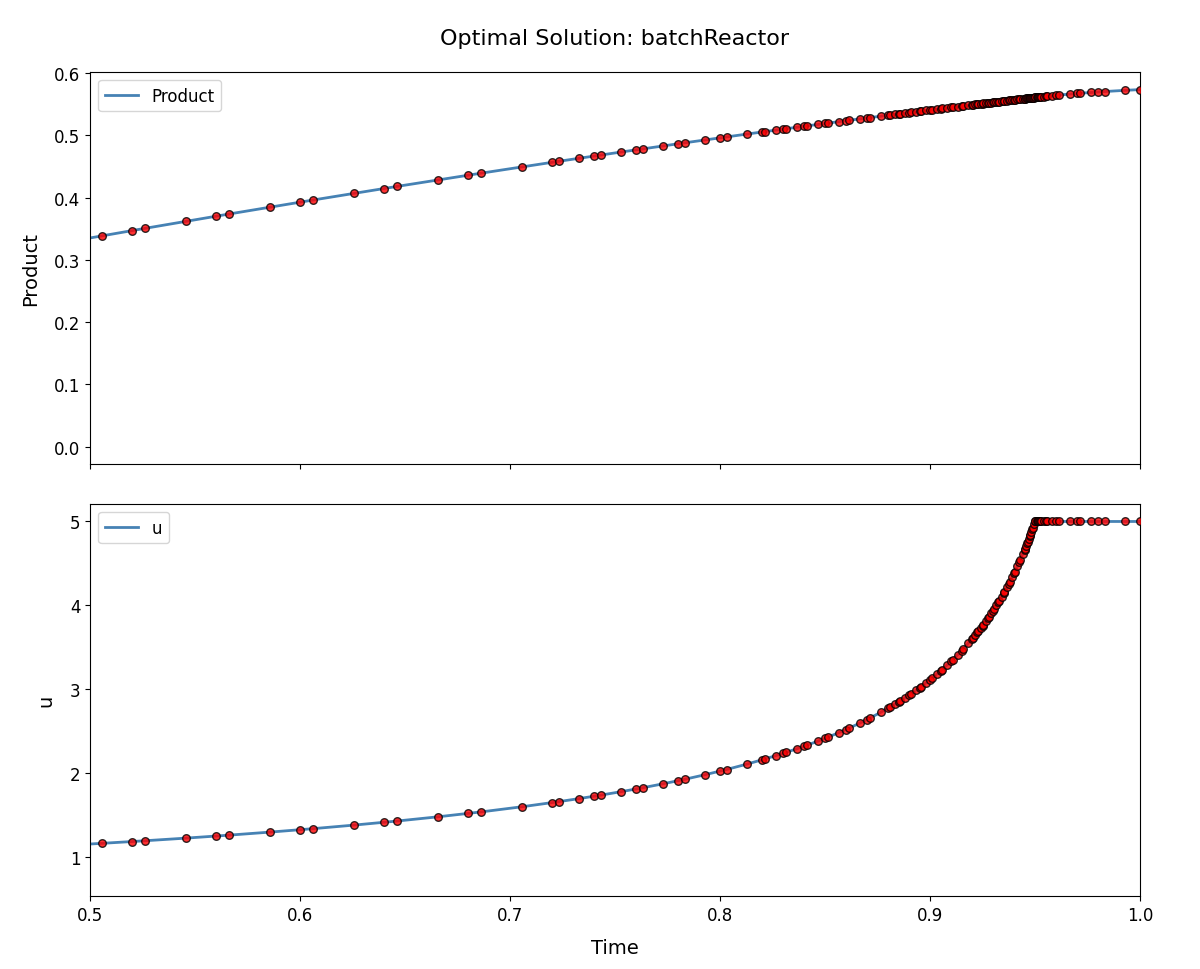
\includegraphics[width=1\textwidth]{images/plotstd.png}
		\caption{Optimal product and control the "Batch Reactor" example}
		\label{fig:batch}
	\end{figure}

\end{mdframed}

\begin{mdframed}[backgroundcolor=gray!10, roundcorner=10pt,
		linewidth=1pt]

	Draws a parametric plot of the optimal solution.

	\begin{lstlisting}
model.parametricPlot(varX, varY, meshIteration=None, interval=None, dots=Dots.OFF)
		\end{lstlisting}
	\label{parametricPlot}
	\textbf{Parameters:}
	\begin{itemize}
		\item \texttt{Symbol varX}: Symbol of the variable on the
		      x-axis.

		\item \texttt{Symbol varY}: Symbol of the variable on the
		      y-axis.

		\item \texttt{int meshIteration} \emph{(optional)}: Sets the
		      mesh iteration of which the optimal values originate. If no value is provided,
		      the last iteration is used.

		\item \texttt{[float, float] interval} \emph{(optional)}: Sets
		      the time range of the plot. Defaults to the interval $[t_0, t_f]$.

		\item \texttt{Dots dots} \emph{(optional)}: Adds dots of the
		      discrete solution to the plot. This has to be an element of the \texttt{Dots}
		      enumeration \eqref{enum:Dots} and in the default case no dots are added.
	\end{itemize}

	\textbf{Example:}
	\begin{lstlisting}
model.parametricPlot(xpos, ypos)   
\end{lstlisting}
\end{mdframed}

\begin{mdframed}[backgroundcolor=gray!10, roundcorner=10pt,
		linewidth=1pt]

	Draws a plot of the mesh refinement process.

	\begin{lstlisting}
model.plotMeshRefinement(interval=None, markerSize=30, dots=Dots.BASE)
		\end{lstlisting}
	\label{plotMeshRefinement}
	\textbf{Parameters:}
	\begin{itemize}
		\item \texttt{[float, float] interval} \emph{(optional)}: Sets
		      the time range of the plot. Defaults to the interval $[t_0, t_f]$.

		\item \texttt{float markerSize} \emph{(optional)}: Sets the
		      size of the dots in the plot.

		\item \texttt{Dots dots} \emph{(optional)}: Sets which points
		      are displayed in the plot. This has to be an element of the \texttt{Dots}
		      enumeration \eqref{enum:Dots} (excluding \texttt{Dots.NONE}) and in the default
		      case base points are added as a dot.
	\end{itemize}

	\textbf{Example:}
	\begin{lstlisting}
model.plotMeshRefinement()
\end{lstlisting}
	\begin{figure}[H]
		\centering
		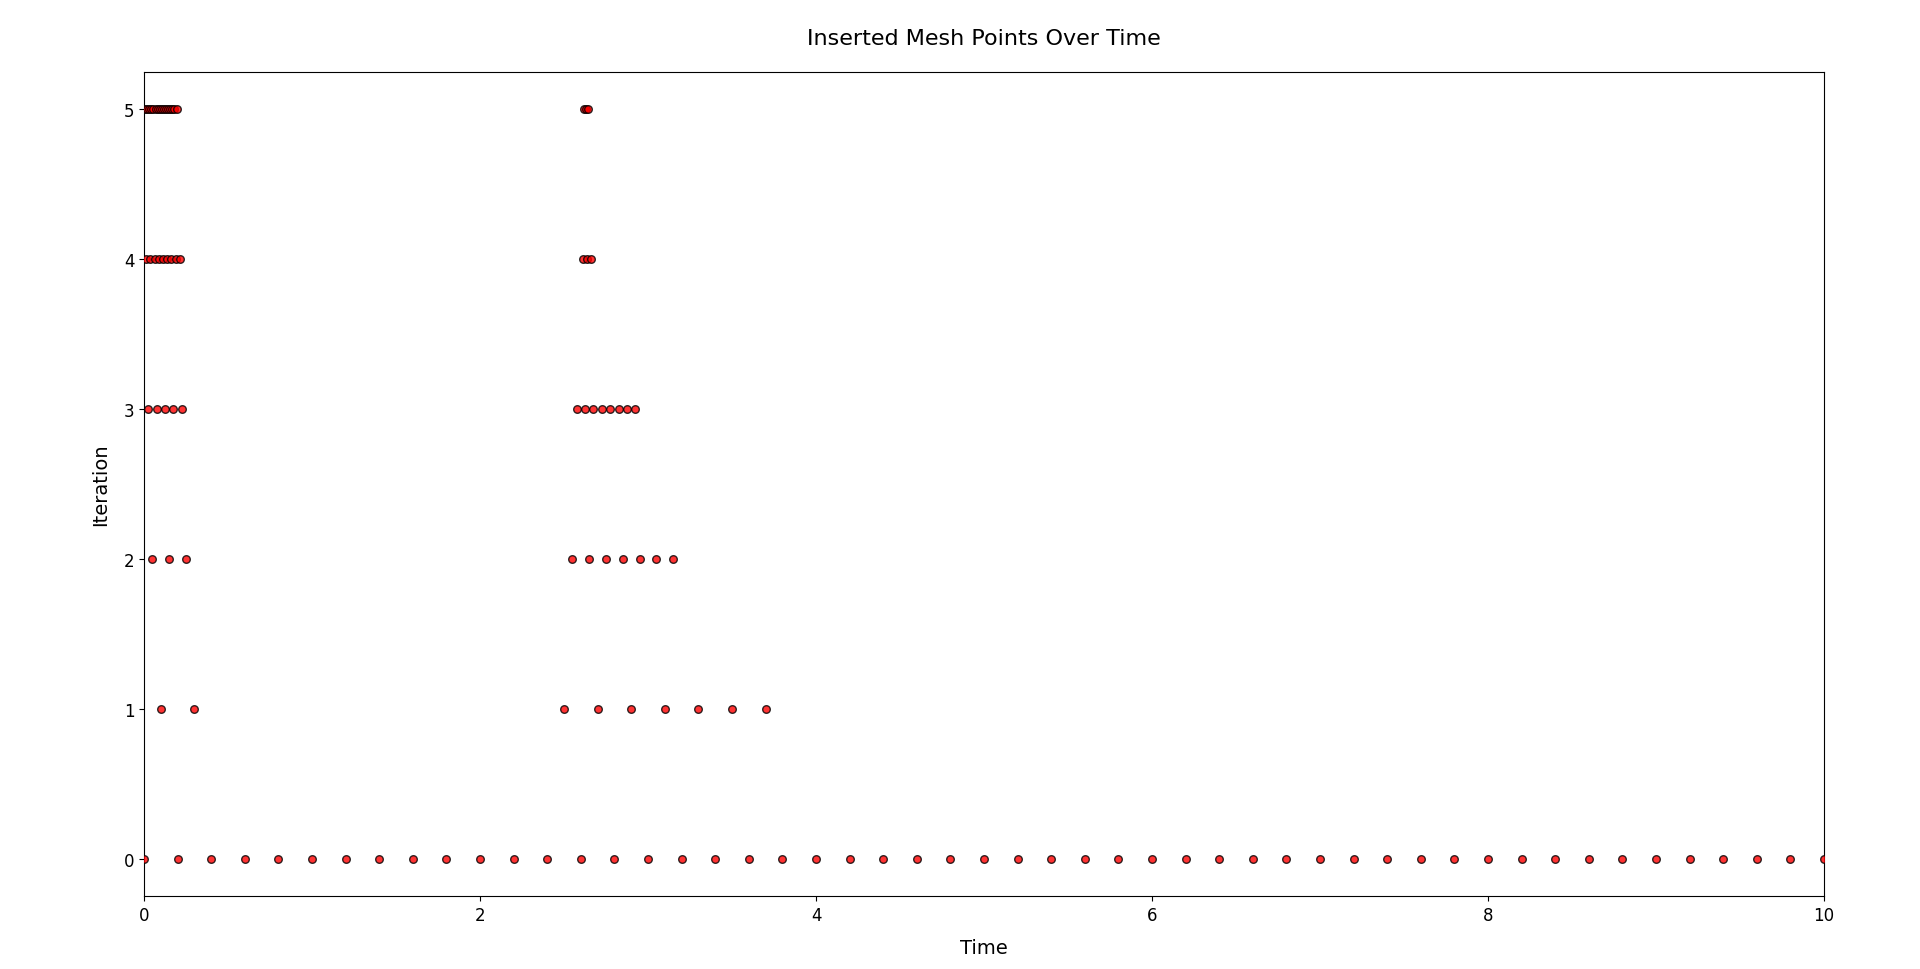
\includegraphics[width=1\textwidth]{images/refinementVDP.png}
		\caption{Mesh refinement in the "Van der Pol" example}
		\label{fig:vdp}
	\end{figure}
\end{mdframed}

The plot of the mesh refinement is not very useful on its own. It is therefore
possible to combine it with standard plots. In this way, the sections that have
been recognized as important or conspicuous by the  algorithm can be
investigated further.

\begin{mdframed}[backgroundcolor=gray!10, roundcorner=10pt,
		linewidth=1pt]

	Draws a combined plot of the mesh refinement and given standard plots.

	\begin{lstlisting}
model.plotVarsAndRefinement(meshIteration=None, interval=None, specifCols=None, markerSize=30, dotsMesh=Dots.BASE, dotsGraph=Dots.OFF)
		\end{lstlisting}
	\label{plotVarsAndRefinement}
	\textbf{Parameters:}
	\begin{itemize}
		\item \texttt{int meshIteration} \emph{(optional)}: Sets the
		      mesh iteration of which the optimal values for the standard plots originate. If
		      no value is provided, the last iteration is used.

		\item \texttt{[float, float] interval} \emph{(optional)}: Sets
		      the time range of the plot. Defaults to the interval $[t_0, t_f]$.

		\item \texttt{list<str> specifCols} \emph{(optional)}: Sets the
		      list of variables that will be drawn. These strings have to match the columns
		      names in \texttt{model.resultHistory} or equivalently the \texttt{symbol}
		      argument of the variables. If no value is provided, all variables will be drawn
		      in the plot.

		\item \texttt{float markerSize} \emph{(optional)}: Sets the
		      size of the dots in the refinement plot.

		\item \texttt{Dots dotsMesh} \emph{(optional)}: Sets which
		      points are displayed in the refinement plot. This has to be an element of the
		      \texttt{Dots} enumeration \eqref{enum:Dots} (excluding \texttt{Dots.NONE}) and
		      in the default case base points are added as a dot.

		\item \texttt{Dots dotsGraph} \emph{(optional)}: Adds dots of
		      the discrete solution to the standard plot. This has to be an element of the
		      \texttt{Dots} enumeration \eqref{enum:Dots} and in the default case no dots are
		      added.
	\end{itemize}

	\textbf{Special cases:}
	There is also a special case for input variables. This shares
	all arguments with \texttt{model.plotVarsAndRefinement}, but only contains the
	plots of the input variables by default.
	\begin{lstlisting}
model.plotInputsAndRefinement(meshIteration=None, interval=None, markerSize=30, dotsMesh=Dots.BASE, dotsGraph=Dots.BASE)    
		\end{lstlisting}

	\textbf{Example:}
	\begin{lstlisting}
model.plotInputsAndRefinement()
\end{lstlisting}
	\begin{figure}[H]
		\centering
		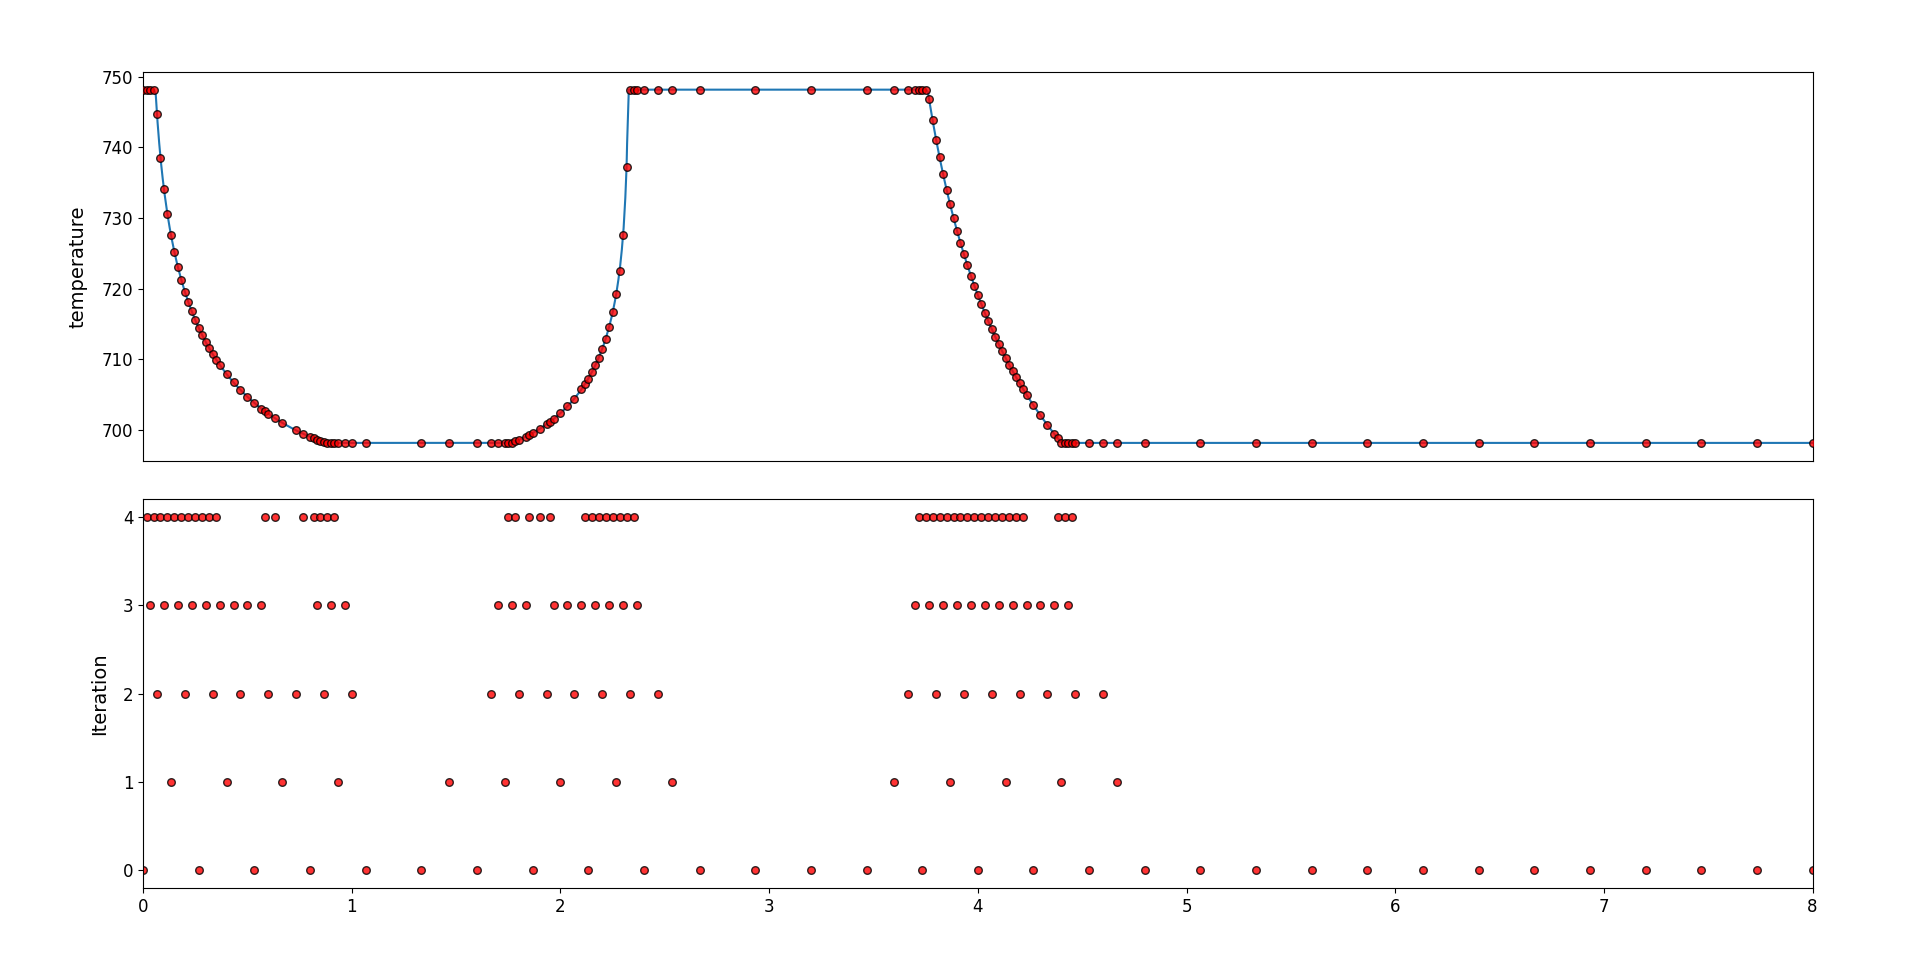
\includegraphics[width=1\textwidth]{images/refinement.png}
		\caption{Mesh refinement and temperature control in an "Oil Shale
			Pyrolysis"}
		\label{fig:osp}
	\end{figure}
\end{mdframed}

Additionally, the framework is capable of drawing sparsity patterns. To be able
to draw a given sparsity pattern the flag \texttt{"exportJacobianPath"}
\eqref{flag:exportJacobianPath} or \texttt{"exportHessianPath"}
\eqref{flag:exportHessianPath} has to be set.

\begin{mdframed}[backgroundcolor=gray!10, roundcorner=10pt,
		linewidth=1pt]

	Draws the Jacobian or Hessian sparsity pattern of the resulting
	large-scale NLP.

	\begin{lstlisting}
model.plotSparseMatrix(matrixType)
		\end{lstlisting}
	\label{plotSparseMatrix}
	\textbf{Parameters:}
	\begin{itemize}
		\item \texttt{MatrixType matrixType}: Sets the matrix. This has
		      to be an element of the \texttt{MatrixType} enumeration
		      \eqref{enum:MatrixType}.
	\end{itemize}

	\textbf{Example:}
	\begin{lstlisting}
model.plotSparseMatrix(MatrixType.JACOBIAN)   
\end{lstlisting}
	\begin{figure}[H]
		\centering
		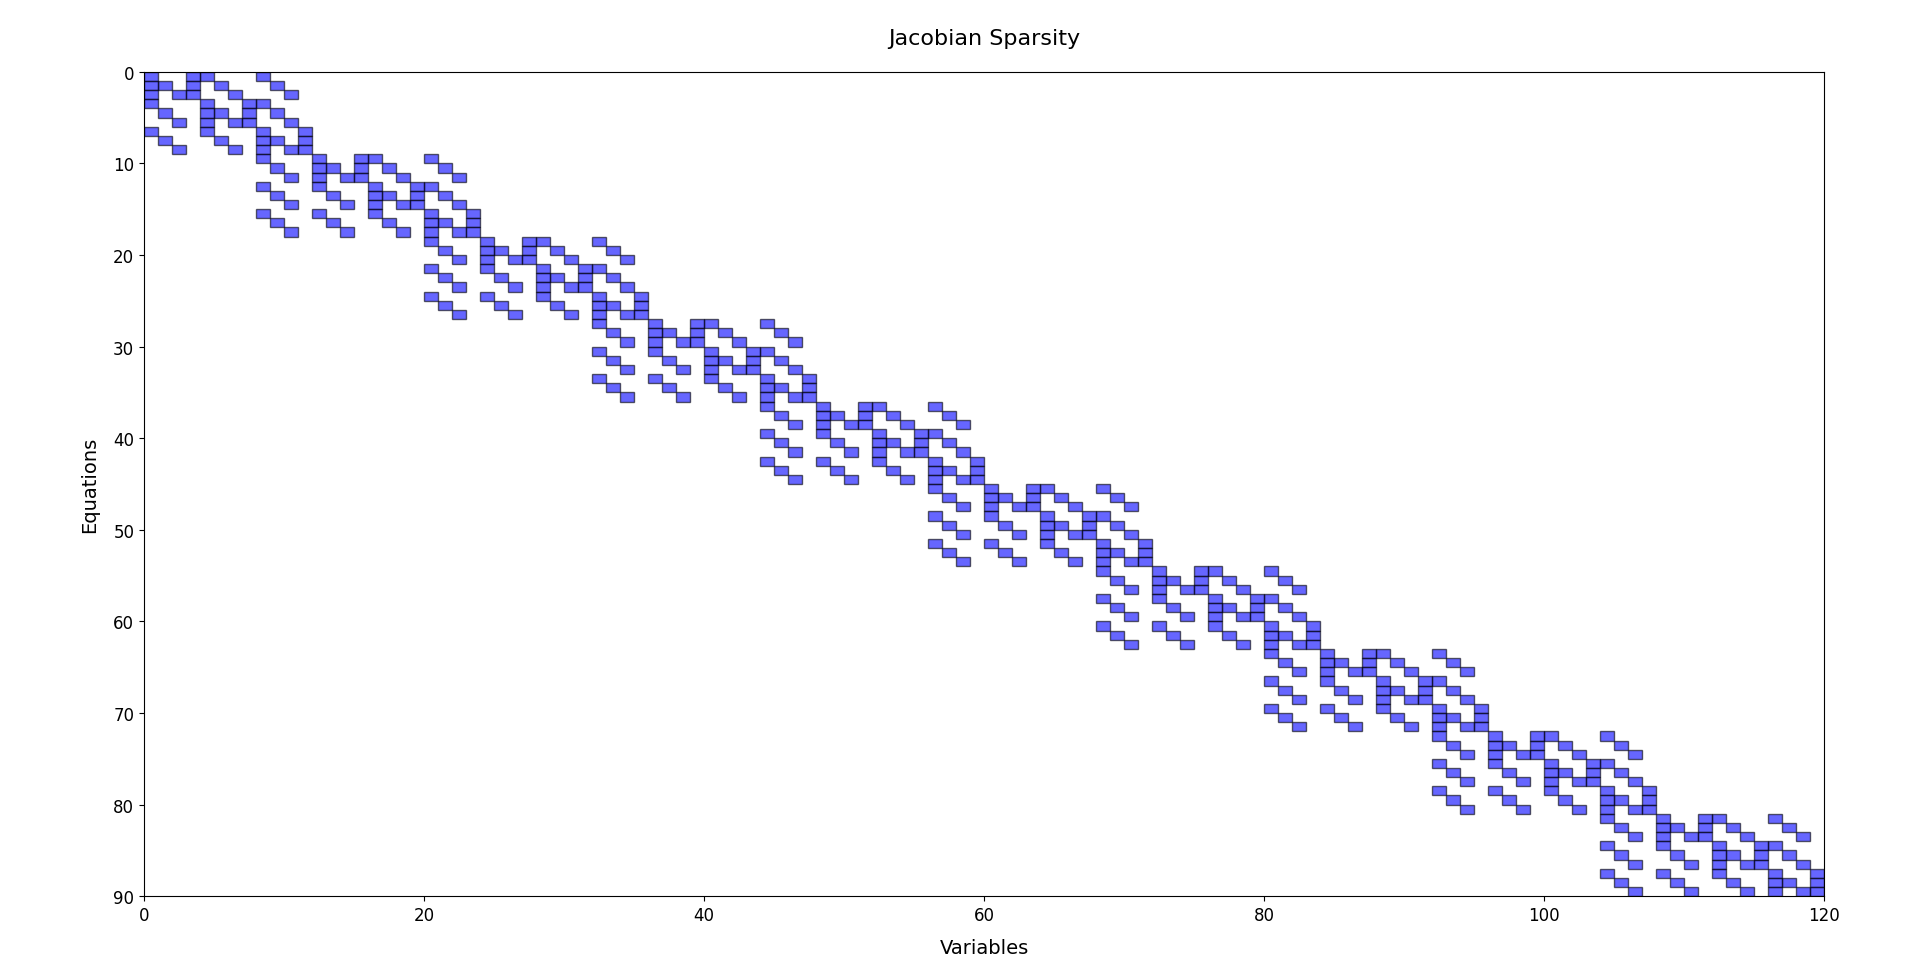
\includegraphics[width=1\textwidth]{images/sparse.png}
		\caption{Jacobian sparsity pattern of the "Batch Reactor" example}
		\label{fig:sparseBatch}
	\end{figure}
\end{mdframed}

\section{Utilities}
The package provides access to many utilities.
These contain special functions, global time symbols and many structures to
obtain more streamlined flags and arguments.

\subsection{Special Functions}
\label{c:specialFunction}
By importing \texttt{gdopt}, some special functions and symbols
get automatically imported from SymEngine. These can be used freely in the
modeling process, although the user has to be careful with non differentiable
and discontinuous functions.
\begin{itemize}
	\item \texttt{exp}, \texttt{log}
	\item \texttt{sin}, \texttt{cos}, \texttt{tan}
	\item \texttt{sqrt}
	\item \texttt{asin}, \texttt{acos}, \texttt{atan}
	\item \texttt{sinh}, \texttt{cosh}, \texttt{tanh}
	\item \texttt{asinh}, \texttt{acosh}, \texttt{atanh}
	\item \texttt{Abs}
	\item \texttt{Max}, \texttt{Min}
	\item \texttt{Piecewise} / \texttt{piecewise}
	\item \texttt{pi}
\end{itemize}

Note that \texttt{Piecewise} is the native SymEngine function to define
piecewise functions. For code generation to work, this function has to have the
fallback
case \texttt{(0, True)}, i.e. the function is constant $0$ anywhere, where it
was not explicitly defined. This inconvenience is addressed with the custom
\texttt{piecewise} function. It is a basic wrapper around \texttt{Piecewise},
where the argument \texttt{(0, True)} is added implicitly. Piecewise functions
allow for greater expressibility in objectives and constraints, e.g.

\begin{lstlisting}
# constraint only has to hold for time < 0.25
binaryTrigger = piecewise((1, t < 0.25), (0, t >= 0.25))
model.addPath(x1 * u1 * binaryTrigger, lb=-30, ub=30) 
\end{lstlisting}

The formulated path constraint is given by
$\begin{cases}
		-30 \leq x_1  u_1 \leq 30, & t < 0.25    \\
		-30 \leq 0 \leq 30,        & t \geq 0.25 \\
	\end{cases}$
and obviously holds for $t \geq 0.25$. It is therefore possible to restrict the
domain of constraints to a subinterval $I \subset [t_0, t_f]$. Piecewise
functions can be useful in many scenarios, e.g. if the Lagrange integrand only
matters on a subset of the entire time horizon, i.e. $\min \int_{t_1}^{t_2}
	L(\cdot) \, \dd t$ with $[t_1, t_2] \subset [t_0, t_f]$.

\subsection{Global Time Symbols}
\label{c:globaltime}
In every \texttt{Model} two global time symbols can be accessed:

\begin{mdframed}[backgroundcolor=gray!10, roundcorner=10pt,
		linewidth=1pt]

	The time symbol can be used in objectives, constraints or in
	input guesses. This represents the time in the model, i.e. $t \in [t_0,
			t_f]$.

	\begin{lstlisting}
t = Symbol("t")
		\end{lstlisting}
	\label{timeSymbol}

	\textbf{Aliases:} \texttt{time}, \texttt{TIME\_SYMBOL}
\end{mdframed}

\begin{mdframed}[backgroundcolor=gray!10, roundcorner=10pt,
		linewidth=1pt]

	The constant final time symbol can be used in objectives,
	constraints, starting values, nominal values, lower and upper bounds,
	etc.
	This represents the final time $t_f$ of the model. The
	associated value will be substituted at runtime.

	\begin{lstlisting}
tf = Symbol("FINAL_TIME")
		\end{lstlisting}
	\label{finalTimeSymbol}

	\textbf{Aliases:} \texttt{finalTime},
	\texttt{FINAL\_TIME\_SYMBOL}
\end{mdframed}

\subsection{Helper Expressions}

Since each expression in the framework is essentially a SymEngine
\texttt{Expression}, the user is able to use so-called helper expressions
throughout the entire modeling process.

E.g. the following dynamic has to be modeled:
\begin{align*}
	\dot{x} & = \exp\left(x + \frac{u}{1 + y^2}\right) + u y \\
	\dot{y} & = \exp\left(x + \frac{u}{1 + y^2}\right) + u x
\end{align*}

By introducing a helper variable, the model becomes way more readable.

\begin{lstlisting}
expTerm = exp(x + u / (1 + y**2))	 # helper expression
model.addDynamic(x, expTerm + u * y)  # simple dynamic for x
model.addDynamic(y, expTerm + u * x)  # simple dynamic for y
	\end{lstlisting}

These helper expressions can also be the Python standard types
\texttt{float} and \texttt{int}. This allows for the modeling of global
constants.

E.g. consider this simple free fall dynamic:
\begin{lstlisting}
g = -9.80665		      # constant gravitational acceleration  
model.addDynamic(v, a + g)  # dynamic using the constant
	\end{lstlisting}

\subsection{Expression Simplification}
If the expressions provided by the user are not simplified yet, it
may be advantageous to enable global expression simplification. This is done by
adding the line
\begin{lstlisting}
model.setExpressionSimplification(True)
	\end{lstlisting}
directly after the creation of the \texttt{Model}.

\subsection{Constant Derivatives}
As mentioned in chapter \eqref{c:collocation} the framework reduces the
continuous formulation of the GDOP \eqref{c:GDOP} to a large scale nonlinear
program (NLP). Since the underlying Solver IPOPT requires the 1st and 2nd
derivatives of this NLP in every iteration, it is beneficial if these
derivatives are constant and thus have to be calculated only once.

The user can call three methods depending on the structure of the
continuous problem formulation. These set the corresponding parameters in
the back-end of the framework and therefore reduce the execution time.

Only call these methods if the requirements are met, otherwise the
Solver converges very slowly or diverges.

\begin{mdframed}[backgroundcolor=gray!10, roundcorner=10pt,
		linewidth=1pt]

	Tells the solver that the Mayer term $M(\v{x}(t_f), \v{u}(t_f),
		\v{p}, t_f)$ and Lagrange integrand $L(\v{x}(t), \v{u}(t),
		\v{p}, t)$ are at
	most linear.

	\begin{lstlisting}
model.hasLinearObjective()
		\end{lstlisting}
	\label{hasLinearObjective}
\end{mdframed}

\begin{mdframed}[backgroundcolor=gray!10, roundcorner=10pt,
		linewidth=1pt]

	Tells the solver that the Mayer term $M(\v{x}(t_f), \v{u}(t_f),
		\v{p}, t_f)$ and Lagrange integrand $L(\v{x}(t), \v{u}(t),
		\v{p}, t)$ are at
	most quadratic.

	\begin{lstlisting}
model.hasQuadraticObjective()
	\end{lstlisting}
	\label{hasQuadraticObjective}

\end{mdframed}

\begin{mdframed}[backgroundcolor=gray!10, roundcorner=10pt,
		linewidth=1pt]

	Tells the solver that all constraints are at most linear, i.e.
	$\v{f}(\cdot), \v{g}(\cdot), \v{r}(\cdot), \v{a}(\cdot)$ are linear or
	constant.

	\begin{lstlisting}
model.hasLinearConstraints()
		\end{lstlisting}
	\label{hasLinearConstraints}

\end{mdframed}

Depending on the above mentioned methods, the following derivatives of
the NLP are assumed to be constant:

\begin{itemize}
	\item Gradient of the objective function, if
	      \texttt{model.hasLinearObjective()}
	\item Jacobian of the constraint vector, if
	      \texttt{model.hasLinearConstraints()}
	\item Hessian of the augmented Lagrangian, if
	      \texttt{model.hasLinearConstraints()} and
	      (\texttt{model.hasLinearObjective()}
	      or \texttt{model.hasQuadraticObjective()})
\end{itemize}

Note that it is also possible to set the flags \texttt{"linearObjective"} \eqref{flag:linearObjective}, \texttt{"quadraticObjective"} \eqref{flag:quadraticObjective}, and \texttt{"linearConstraints"} \eqref{flag:linearConstraints} to tell the solver that constant derivatives are present.

\subsection{Enumerations}

\subsubsection{Objective}
\begin{mdframed}[backgroundcolor=gray!10, roundcorner=10pt,
		linewidth=1pt]
	Enumeration for the attribute \texttt{obj} of
	\texttt{model.addMayer} \eqref{addMayer}, \texttt{model.addLagrange}
	\eqref{addLagrange}, and \texttt{model.addObjective}
	\eqref{addObjective}:
	Objective goal.

	\begin{lstlisting}
Objective(Enum)
		\end{lstlisting}
	\label{enum:Objective}
	\textbf{Elements:}
	\begin{itemize}
		\item \texttt{MINIMIZE}: Minimize the objective.
		\item \texttt{MAXIMIZE}: Maximize the objective. Will
		      multiply the provided expression with a factor of $-1$,
		      since the optimizer
		      minimizes.

	\end{itemize}

	\textbf{Aliases:} \texttt{MIN} = \texttt{MINIMIZE},
	\texttt{MAX} = \texttt{MAXIMIZE}

\end{mdframed}

\subsubsection{LinearSolver}

\begin{mdframed}[backgroundcolor=gray!10, roundcorner=10pt,
		linewidth=1pt]
	Enumeration for the flag \texttt{"linearSolver"}
	\eqref{flag:linearSolver}:
	Specifies the linear solver used by IPOPT.

	\begin{lstlisting}
LinearSolver(Enum)
	\end{lstlisting}
	\label{enum:LinearSolver}
	\textbf{Elements:}
	\begin{itemize}
		\item \texttt{MUMPS}: MUMPS.
		\item \texttt{MA27}: MA27 (HSL solver).
		\item \texttt{MA57}: MA57 (HSL solver).
		\item \texttt{MA77}: MA77 (HSL solver).
		\item \texttt{MA86}: MA86 (HSL solver).
		\item \texttt{MA97}: MA97 (HSL solver).
		\item \texttt{PARDISO}: Intel PARDISO (currently not
		      supported).
	\end{itemize}

\end{mdframed}

\subsubsection{InitVars}
\begin{mdframed}[backgroundcolor=gray!10, roundcorner=10pt,
		linewidth=1pt]
	Enumeration for the flag \texttt{"initVars"}
	\eqref{flag:initVars}:
	Determines how the initial solutions for the state
	trajectories, that have to be provided to the nonlinear solver, are
	calculated.

	Note that the initial guess for the parameters and input
	trajectories are given by the \texttt{guess} argument in
	\texttt{model.addInput} \eqref{addInput} and
	\texttt{model.addParameter}
	\eqref{addParameter} respectively.

	\begin{lstlisting}
InitVars(Enum)
	\end{lstlisting}
	\label{enum:initVars}
	\textbf{Elements:}
	\begin{itemize}
		\item \texttt{CONST}: The initial states are given by
		      $\v{x}(t) \equiv \v{x}_0$.
		\item \texttt{SOLVE}: The initial states are computed by
		      solving the dynamic using the guesses for
		      $\v{u}(t)$ and $\v{p}$.
		      The system is solved by
		      \texttt{scipy.integrate.solve\_ivp}. The corresponding
		      \texttt{SciPy} integrator can be set with
		      \eqref{flag:ivpSolver}, which can be
		      implicit.
		\item \texttt{SOLVE\_EXPLICIT}: The initial states are
		      computed by solving the dynamic using the guesses for
		      $\v{u}(t)$ and
		      $\v{p}$. The system is solved by the classic Runge–Kutta
		      method.
		\item \texttt{SOLVE\_EXPLICIT\_EULER}: The initial
		      states are computed by solving the dynamic using the
		      guesses for $\v{u}(t)$
		      and $\v{p}$. The system is solved by the explicit /
		      forward Euler method.

	\end{itemize}

\end{mdframed}

\subsubsection{IVPSolver}

\begin{mdframed}[backgroundcolor=gray!10, roundcorner=10pt,
		linewidth=1pt]
	Enumeration for the flag \texttt{"ivpSolver"}
	\eqref{flag:ivpSolver}:
	Sets the \texttt{SciPy} integrator. If the flag
	\texttt{"initVars"} \eqref{flag:initVars} is set to
	\texttt{InitVars.SOLVE}, this
	integrator is used to solve the dynamic and compute an initial state
	solution.

	\begin{lstlisting}
IVPSolver(Enum)
		\end{lstlisting}
	\label{enum:IVPSolver}
	\textbf{Elements:}
	\begin{itemize}
		\item \texttt{Radau}: RadauIIA of order 5.
		\item \texttt{BDF}: Implicit multi-step of
		      variable-order (1 to 5).
		\item \texttt{LSODA}: Adams/BDF method.
		\item \texttt{DOP853}: Explicit Runge-Kutta method of
		      order 8.
		\item \texttt{RK45}: Explicit Runge-Kutta method of
		      order 5(4).
		\item \texttt{RK23}: Explicit Runge-Kutta method of
		      order 3(2).
	\end{itemize}

	\textbf{Aliases:} \texttt{RADAU} = \texttt{Radau}
\end{mdframed}

\subsubsection{MeshAlgorithm}

\begin{mdframed}[backgroundcolor=gray!10, roundcorner=10pt,
		linewidth=1pt]
	Enumeration for the mesh flag \texttt{"algorithm"}
	\eqref{flag:MeshAlgorithm}:
	Sets the mesh algorithm.

	\begin{lstlisting}
MeshAlgorithm(Enum)
		\end{lstlisting}
	\label{enum:MeshAlgorithm}
	\textbf{Elements:}
	\begin{itemize}
		\item \texttt{NONE}: No mesh algorithm at all.
		\item \texttt{BASIC}: A very basic mesh algorithm, which is
		      based on the deviation of input variables to its mean.
		\item \texttt{L2\_BOUNDARY\_NORM}: An advanced mesh algorithm,
		      which is based on evaluating specific L2-norms and
		      comparing derivatives at the
		      interval boundaries. This algorithm is able to detect
		      jumps, steep sections and
		      corners, while being
		      computationally inexpensive.
	\end{itemize}

\end{mdframed}

\subsubsection{RefinementMethod}

\begin{mdframed}[backgroundcolor=gray!10, roundcorner=10pt,
		linewidth=1pt]
	Enumeration for the mesh flag \texttt{"refinementMethod"}
	\eqref{flag:RefinementMethod}:
	Sets the refinement method, which determines how the initial values for
	$\v{x}(t)$ and $\v{u}(t)$ are evaluated from the previous iteration, if
	a mesh refinement is executed.

	\begin{lstlisting}
RefinementMethod(Enum)
	\end{lstlisting}
	\label{enum:RefinementMethod}
	\textbf{Elements:}
	\begin{itemize}
		\item \texttt{LINEAR\_SPLINE}: The variables are being
		      interpolated by a linear spline on each interval. The
		      initial solution
		      should contain no oscillations at discontinuities, but
		      might be poor for smooth
		      sections.
		\item \texttt{POLYNOMIAL}: The variables are being
		      interpolated by an interpolating polynomial on each
		      interval.
		      The initial solution
		      is likely to contain oscillations at discontinuities,
		      although
		      being advantageous for smooth
		      sections.
	\end{itemize}

\end{mdframed}

\subsubsection{MatrixType}
\label{c:MatrixType}
\begin{mdframed}[backgroundcolor=gray!10, roundcorner=10pt,
		linewidth=1pt]
	Enumeration that specifies a sparse matrix, i.e. Jacobian or Hessian.

	\begin{lstlisting}
MatrixType(Enum)
	\end{lstlisting}
	\label{enum:MatrixType}
	\textbf{Elements:}
	\begin{itemize}
		\item \texttt{JACOBIAN}: Jacobian matrix.
		\item \texttt{HESSIAN}: Hessian matrix.
	\end{itemize}

\end{mdframed}

\subsubsection{Dots}
\label{c:Dots}
\begin{mdframed}[backgroundcolor=gray!10, roundcorner=10pt,
		linewidth=1pt]
	Enumeration for the \texttt{dots} argument in all plotting methods.
	\eqref{c:Plotting} Determines if and which values are added to the plot
	as a dot.

	\begin{lstlisting}
Dots(Enum)
	\end{lstlisting}
	\label{enum:Dots}
	\textbf{Elements:}
	\begin{itemize}
		\item \texttt{OFF}: No dots are added to the plot.
		\item \texttt{ALL}: The state and input values at all grid
		      points are added to the plot.
		\item \texttt{BASE}: The state and input values at the base
		      point of each interval are added to the plot.
	\end{itemize}

\end{mdframed}
\newpage
\section{Example Code}

Note that the previously mentioned GitHub repository offers many more examples
to get an easy introduction to modeling with this framework. Nevertheless some
basic and instructive examples are also provided in this User's Guide.

\subsection{Batch Reactor}

\begin{lstlisting}
from gdopt import *

"""
* Batch Reactor from Parallel Multiple-Shooting and Collocation Optimization with OpenModelica,
* Bachmann, Ochel, et. al., 2012
"""

model = Model("batchReactor")

x1 = model.addState(symbol="Reactant", start=1)
x2 = model.addState(symbol="Product", start=0)

# a non trivial guess for the control variable
controlGuess = guessPiecewise((0.7, t <= 1/2),
			         (guessQuadratic(0.6, 0.7, 5), 1/2 < t))
u = model.addControl(symbol="u", lb=0, ub=5, guess=controlGuess)

model.addDynamic(x1, -(u + u**2 / 2) * x1)
model.addDynamic(x2, u * x1)

model.addMayer(x2, Objective.MAXIMIZE)

model.hasLinearObjective()

model.generate()

model.optimize(tf=1, steps=250, rksteps=3,
	flags={
		"outputPath": "/tmp",
		"linearSolver": LinearSolver.MUMPS,
		"initVars": InitVars.SOLVE
	},
	meshFlags={
		"algorithm": MeshAlgorithm.L2_BOUNDARY_NORM,
		"iterations": 6
	}
)
model.printResults()
model.plotInputsAndRefinement()

\end{lstlisting}
\newpage
\subsection{Oil Shale Pyrolysis}

\begin{lstlisting}
from gdopt import *

model = Model("oilShalePyrolysis")

x1 = model.addState(start=1, symbol="kerogen")
x2 = model.addState(start=0, symbol="bitumen")
x3 = model.addState(start=0, symbol="oil")
x4 = model.addState(start=0, symbol="carbon")

T = model.addInput(lb=698.15, ub=748.15, symbol="temperature")

k1 = exp(8.86 - (20300 / 1.9872) / T)
k2 = exp(24.25 - (37400 / 1.9872) / T)
k3 = exp(23.67 - (33800 / 1.9872) / T)
k4 = exp(18.75 - (28200 / 1.9872) / T)
k5 = exp(20.70 - (31000 / 1.9872) / T)

model.addDynamic(x1, -k1 * x1 - (k3 + k4 + k5) * x1 * x2)
model.addDynamic(x2, k1 * x1 - k2 * x2 + k3 * x1 * x2)
model.addDynamic(x3, k2 * x2 + k4 * x1 * x2)
model.addDynamic(x4, k5 * x1 * x2)

model.addMayer(x2, Objective.MAXIMIZE)

model.generate()

model.optimize(
	tf=8,
	steps=200,
	rksteps=3,
	flags={
		"outputPath": "/tmp",
		"tolerance": 1e-14,
	        "linearSolver": LinearSolver.MA57
        },
	meshFlags={
		"algorithm": MeshAlgorithm.L2_BOUNDARY_NORM,
		"iterations": 5
	}
)

model.printResults()
model.plot()
\end{lstlisting}
\newpage
\subsection{Van der Pol Oscillator}

\begin{lstlisting}
from gdopt import *

model = Model("vanDerPol")

x1 = model.addState(start=0)
x2 = model.addState(start=1)

u = model.addInput(ub=0.8)

rp = model.addRuntimeParameter(default=1, symbol="RP")

model.addDynamic(x1, (1 - x2**2) * x1 - x2 + u)
model.addDynamic(x2, x1)

model.addLagrange(x1**2 + x2**2 + rp * u**2)

model.generate()

model.optimize(
	tf=10,
	steps=50,
	rksteps=3,
	flags={
		"outputPath": "/tmp",
		"linearSolver": LinearSolver.MUMPS
	},
	meshFlags={
		"algorithm": MeshAlgorithm.L2_BOUNDARY_NORM,
		"iterations": 5,
		"refinementMethod": RefinementMethod.POLYNOMIAL
	}
)

model.parametricPlot(x1, x2, dots=Dots.BASE)

model.setValue(rp, 0.1)

model.optimize(resimulate=True)
model.plotInputsAndRefinement()
\end{lstlisting}
\newpage
\subsection{Nominal Batch Reactor}

\begin{lstlisting}	
from gdopt import *

model = Model("nominalBatchReactor")

NOM = model.addRuntimeParameter(default=1e-10, symbol="NOM")

y1 = model.addState(symbol="Reactant", start=NOM, nominal=NOM)
y2 = model.addState(symbol="Product", start=0, nominal=1 / NOM)

u = model.addInput(symbol="u", lb=0, ub=5, guess=1)

x1 = y1 / NOM
x2 = y2 * NOM

model.addDynamic(y1, -(u + u**2 / 2) * x1 * NOM, nominal=NOM)
model.addDynamic(y2, u * x1 / NOM, nominal=1 / NOM)

model.addMayer(y2, Objective.MAXIMIZE, nominal=1 / NOM)

model.hasLinearObjective()

model.generate()

model.optimize(
tf=1,
steps=500,
rksteps=3,
flags={"outputPath": "/tmp", "linearSolver": LinearSolver.MA57, "initVars": InitVars.SOLVE, "tolerance": 1e-14},
)

model.setValue(NOM, 1e10)
model.optimize(resimulate=True)

model.plot(dots=Dots.BASE)


\end{lstlisting}

\newpage
\fancyhead[R]{}
\thispagestyle{fancy}

\begin{thebibliography}{9}

	\bibitem{wachter2006implementation}
	Wächter, A. and L. T. Biegler, “On the Implementation of an
	Interior-Point Filter Line-Search Algorithm for Large-Scale Nonlinear
	Programming”, \textit{Mathematical Programming}, 106(1):25-57, 2006.

	\bibitem{amestoy2001fully}
	Amestoy, P. R., Duff, I. S., L’Excellent, J.-Y., \& Koster, J. (2001).
	A fully asynchronous multifrontal solver using distributed dynamic scheduling.
	\textit{SIAM Journal on Matrix Analysis and Applications}, 23(1), 15-41.

	\bibitem{hsl2013collection}
	HSL. (2013). A collection of Fortran codes for large-scale scientific
	computation. \url{http://www.hsl.rl.ac.uk}.

	\bibitem{symengine}
	SymEngine Developers,
	\textit{SymEngine: A Fast Symbolic Manipulation Library},
	GitHub repository,
	\url{https://github.com/symengine/symengine},
	accessed September 27, 2024.

	\bibitem{harris2020array}
	Harris, C. R., Millman, K. J., et al. (2020). Array programming with
	NumPy. \textit{Nature}, 585(7825), 357-362.

	\bibitem{virtanen2020scipy}
	Virtanen, P., et al. (2020). SciPy 1.0: Fundamental algorithms for
	scientific computing in Python. \textit{Nature Methods}, 17(3), 261-272.

	\bibitem{mckinney2010data}
	McKinney, W. (2010). Data structures for statistical computing in
	Python. In \textit{Proceedings of the 9th Python in Science Conference} (Vol.
	445, pp. 51-56).

	\bibitem{hunter2007matplotlib}
	Hunter, J. D. (2007). Matplotlib: A 2D graphics environment.
	\textit{Computing in Science} \& \textit{Engineering}, 9(3), 90-95.

	\bibitem{openmodelica}
	OpenModelica. (n.d.). OpenModelica User's Guide. Retrieved from
	\url{https://openmodelica.org/doc/OpenModelicaUsersGuide/latest/optimization.html}.

\end{thebibliography}

\end{document}
